\documentclass[12pt]{beamer}\usepackage[]{graphicx}\usepackage[]{color}
%% maxwidth is the original width if it is less than linewidth
%% otherwise use linewidth (to make sure the graphics do not exceed the margin)
\makeatletter
\def\maxwidth{ %
  \ifdim\Gin@nat@width>\linewidth
    \linewidth
  \else
    \Gin@nat@width
  \fi
}
\makeatother

\definecolor{fgcolor}{rgb}{0.345, 0.345, 0.345}
\newcommand{\hlnum}[1]{\textcolor[rgb]{0.686,0.059,0.569}{#1}}%
\newcommand{\hlstr}[1]{\textcolor[rgb]{0.192,0.494,0.8}{#1}}%
\newcommand{\hlcom}[1]{\textcolor[rgb]{0.678,0.584,0.686}{\textit{#1}}}%
\newcommand{\hlopt}[1]{\textcolor[rgb]{0,0,0}{#1}}%
\newcommand{\hlstd}[1]{\textcolor[rgb]{0.345,0.345,0.345}{#1}}%
\newcommand{\hlkwa}[1]{\textcolor[rgb]{0.161,0.373,0.58}{\textbf{#1}}}%
\newcommand{\hlkwb}[1]{\textcolor[rgb]{0.69,0.353,0.396}{#1}}%
\newcommand{\hlkwc}[1]{\textcolor[rgb]{0.333,0.667,0.333}{#1}}%
\newcommand{\hlkwd}[1]{\textcolor[rgb]{0.737,0.353,0.396}{\textbf{#1}}}%
\let\hlipl\hlkwb

\usepackage{framed}
\makeatletter
\newenvironment{kframe}{%
 \def\at@end@of@kframe{}%
 \ifinner\ifhmode%
  \def\at@end@of@kframe{\end{minipage}}%
  \begin{minipage}{\columnwidth}%
 \fi\fi%
 \def\FrameCommand##1{\hskip\@totalleftmargin \hskip-\fboxsep
 \colorbox{shadecolor}{##1}\hskip-\fboxsep
     % There is no \\@totalrightmargin, so:
     \hskip-\linewidth \hskip-\@totalleftmargin \hskip\columnwidth}%
 \MakeFramed {\advance\hsize-\width
   \@totalleftmargin\z@ \linewidth\hsize
   \@setminipage}}%
 {\par\unskip\endMakeFramed%
 \at@end@of@kframe}
\makeatother

\definecolor{shadecolor}{rgb}{.97, .97, .97}
\definecolor{messagecolor}{rgb}{0, 0, 0}
\definecolor{warningcolor}{rgb}{1, 0, 1}
\definecolor{errorcolor}{rgb}{1, 0, 0}
\newenvironment{knitrout}{}{} % an empty environment to be redefined in TeX

\usepackage{alltt}
\usepackage{graphicx}
\usepackage{tikz}
\setbeameroption{hide notes}
\setbeamertemplate{note page}[plain]
\usepackage{listings}

% get rid of junk
\usetheme{default}
\usefonttheme[onlymath]{serif}
\beamertemplatenavigationsymbolsempty
\hypersetup{pdfpagemode=UseNone} % don't show bookmarks on initial view

% named colors
\definecolor{offwhite}{RGB}{255,250,240}
\definecolor{gray}{RGB}{155,155,155}

\ifx\notescolors\undefined % slides

  \definecolor{foreground}{RGB}{80,80,80}
  \definecolor{background}{RGB}{255,255,255}
  \definecolor{title}{RGB}{255,199,0}
  \definecolor{subtitle}{RGB}{89,132,212}
  \definecolor{hilit}{RGB}{248,117,79}
  \definecolor{vhilit}{RGB}{255,111,207}
  \definecolor{lolit}{RGB}{200,200,200}
  \definecolor{lit}{RGB}{255,199,0}
  \definecolor{mdlit}{RGB}{89,132,212}
  \definecolor{link}{RGB}{248,117,79}

\else % notes
  \definecolor{background}{RGB}{255,255,255}
  \definecolor{foreground}{RGB}{24,24,24}
  \definecolor{title}{RGB}{27,94,134}
  \definecolor{subtitle}{RGB}{22,175,124}
  \definecolor{hilit}{RGB}{122,0,128}
  \definecolor{vhilit}{RGB}{255,0,128}
  \definecolor{lolit}{RGB}{95,95,95}
\fi
\definecolor{nhilit}{RGB}{128,0,128}  % hilit color in notes
\definecolor{nvhilit}{RGB}{255,0,128} % vhilit for notes

\newcommand{\hilit}{\color{hilit}}
\newcommand{\vhilit}{\color{vhilit}}
\newcommand{\nhilit}{\color{nhilit}}
\newcommand{\nvhilit}{\color{nvhilit}}
\newcommand{\lit}{\color{lit}}
\newcommand{\mdlit}{\color{mdlit}}
\newcommand{\lolit}{\color{lolit}}

% use those colors
\setbeamercolor{titlelike}{fg=title}
\setbeamercolor{subtitle}{fg=subtitle}
\setbeamercolor{frametitle}{fg=gray}
\setbeamercolor{structure}{fg=subtitle}
\setbeamercolor{institute}{fg=lolit}
\setbeamercolor{normal text}{fg=foreground,bg=background}
%\setbeamercolor{item}{fg=foreground} % color of bullets
%\setbeamercolor{subitem}{fg=hilit}
%\setbeamercolor{itemize/enumerate subbody}{fg=lolit}
\setbeamertemplate{itemize subitem}{{\textendash}}
\setbeamerfont{itemize/enumerate subbody}{size=\footnotesize}
\setbeamerfont{itemize/enumerate subitem}{size=\footnotesize}

% center title of slides
\setbeamertemplate{blocks}[rounded]
\setbeamertemplate{frametitle}[default][center]
% margins
\setbeamersize{text margin left=25pt,text margin right=25pt}

% page number
\setbeamertemplate{footline}{%
    \raisebox{5pt}{\makebox[\paperwidth]{\hfill\makebox[20pt]{\lolit
          \scriptsize\insertframenumber}}}\hspace*{5pt}}

% add a bit of space at the top of the notes page
\addtobeamertemplate{note page}{\setlength{\parskip}{12pt}}

% default link color
\hypersetup{colorlinks, urlcolor={link}}

\ifx\notescolors\undefined % slides
  % set up listing environment
  \lstset{language=bash,
          basicstyle=\ttfamily\scriptsize,
          frame=single,
          commentstyle=,
          backgroundcolor=\color{darkgray},
          showspaces=false,
          showstringspaces=false
          }
\else % notes
  \lstset{language=bash,
          basicstyle=\ttfamily\scriptsize,
          frame=single,
          commentstyle=,
          backgroundcolor=\color{offwhite},
          showspaces=false,
          showstringspaces=false
          }
\fi

% a few macros
\newcommand{\code}[1]{\texttt{#1}}
\newcommand{\hicode}[1]{{\hilit \texttt{#1}}}
\newcommand{\bb}[1]{\begin{block}{#1}}
\newcommand{\eb}{\end{block}}
\newcommand{\bi}{\begin{itemize}}
%\newcommand{\bbi}{\vspace{24pt} \begin{itemize} \itemsep8pt}
\newcommand{\bbi}{\vspace{4pt} \begin{itemize} \itemsep8pt}
\newcommand{\ei}{\end{itemize}}
\newcommand{\bv}{\begin{verbatim}}
\newcommand{\ev}{\end{verbatim}}
\newcommand{\ig}{\includegraphics}
\newcommand{\subt}[1]{{\footnotesize \color{subtitle} {#1}}}
\newcommand{\ttsm}{\tt \small}
\newcommand{\ttfn}{\tt \footnotesize}
\newcommand{\figh}[2]{\centerline{\includegraphics[height=#2\textheight]{#1}}}
\newcommand{\figw}[2]{\centerline{\includegraphics[width=#2\textwidth]{#1}}}



%------------------------------------------------
% end of header
%------------------------------------------------

\title{Colors in R}
\subtitle{STAT 133}
\author{\href{http://www.gastonsanchez.com}{Gaston Sanchez}}
\institute{\href{https://github.com/ucb-stat133/stat133-fall-2016}{\tt \scriptsize \color{foreground} github.com/ucb-stat133/stat133-fall-2016}}
\date{}
\IfFileExists{upquote.sty}{\usepackage{upquote}}{}
\begin{document}


{
  \setbeamertemplate{footline}{} % no page number here
  \frame{
    \titlepage
  } 
}

%------------------------------------------------

\begin{frame}
\begin{center}
\Huge{\hilit{Colors in R}}
\end{center}
\end{frame}

%------------------------------------------------

\begin{frame}
\frametitle{Colors in plots}

\bb{Colors on objects}
In R plots, many objects can take on different colors
\bi
  \item points
  \item lines
  \item axes (and tick marks)
  \item filling areas
  \item borders
  \item text
  \item legends
  \item background
 \ei
\eb

\end{frame}

%------------------------------------------------

\begin{frame}[fragile]
\frametitle{Colored points}

\begin{knitrout}\scriptsize
\definecolor{shadecolor}{rgb}{0.969, 0.969, 0.969}\color{fgcolor}\begin{kframe}
\begin{alltt}
\hlstd{x} \hlkwb{<-} \hlopt{-}\hlnum{4}\hlopt{:}\hlnum{4}
\hlstd{y} \hlkwb{<-} \hlstd{x}\hlopt{^}\hlnum{2}
\hlkwd{plot}\hlstd{(x, y,} \hlkwc{pch} \hlstd{=} \hlnum{19}\hlstd{,} \hlkwc{cex} \hlstd{=} \hlnum{3}\hlstd{,} \hlkwc{col} \hlstd{=} \hlkwd{rainbow}\hlstd{(}\hlkwd{length}\hlstd{(x)))}
\end{alltt}
\end{kframe}

{\centering 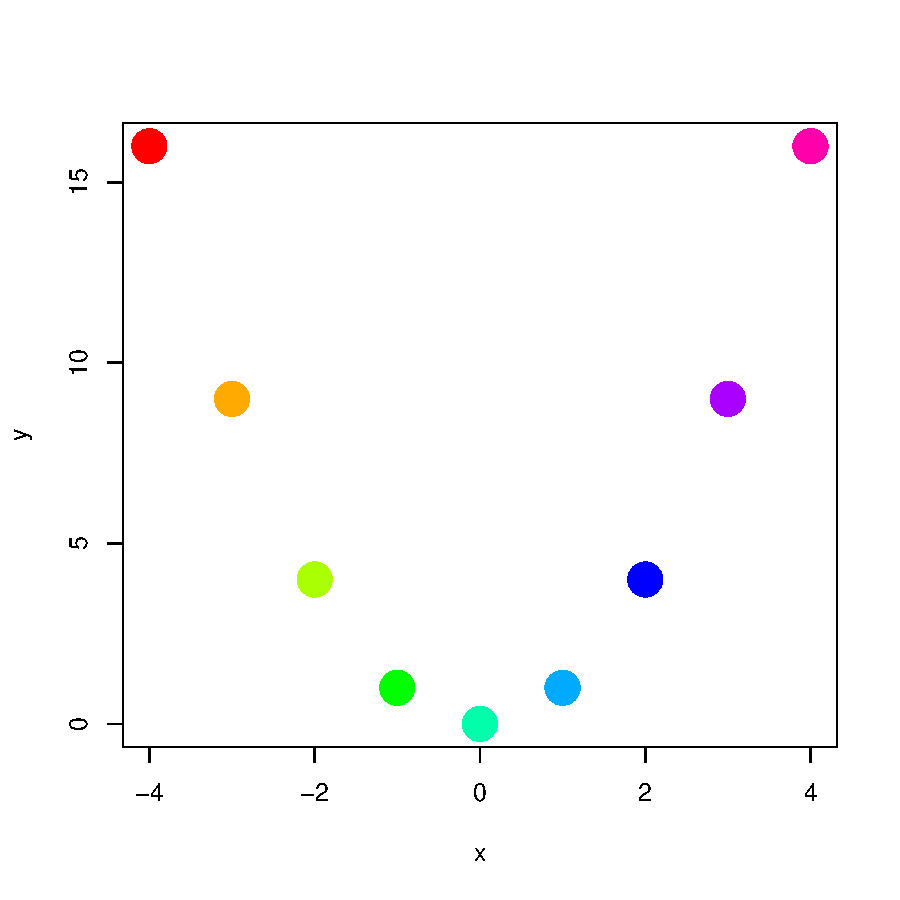
\includegraphics[width=.4\linewidth,height=.4\linewidth]{figure/points_colored1-1} 

}



\end{knitrout}

\end{frame}

%------------------------------------------------

\begin{frame}[fragile]
\frametitle{Colored lines}

\begin{knitrout}\scriptsize
\definecolor{shadecolor}{rgb}{0.969, 0.969, 0.969}\color{fgcolor}\begin{kframe}
\begin{alltt}
\hlcom{# data}
\hlstd{Time} \hlkwb{<-} \hlnum{0}\hlopt{:}\hlnum{120}
\hlstd{Period1} \hlkwb{<-} \hlkwd{cos}\hlstd{(}\hlnum{2} \hlopt{*} \hlstd{pi} \hlopt{*} \hlstd{Time}\hlopt{/}\hlnum{120}\hlstd{)}
\hlstd{Period2} \hlkwb{<-} \hlkwd{cos}\hlstd{(}\hlnum{2} \hlopt{*} \hlstd{pi} \hlopt{*} \hlstd{Time}\hlopt{/}\hlnum{90}\hlstd{)}
\hlstd{Period3} \hlkwb{<-} \hlkwd{cos}\hlstd{(}\hlnum{2} \hlopt{*} \hlstd{pi} \hlopt{*} \hlstd{Time}\hlopt{/}\hlnum{150}\hlstd{)}
\hlstd{Periods} \hlkwb{<-} \hlkwd{data.frame}\hlstd{(}
  \hlkwc{Period1} \hlstd{= Period1,}
  \hlkwc{Period2} \hlstd{= Period2,}
  \hlkwc{Period3} \hlstd{= Period3)}

\hlcom{# graphical parameters}
\hlstd{line_cols} \hlkwb{<-} \hlkwd{c}\hlstd{(}\hlstr{"#5984d4"}\hlstd{,} \hlstr{"#d45984"}\hlstd{,} \hlstr{"#84d459"}\hlstd{)}
\hlstd{line_types} \hlkwb{<-} \hlkwd{c}\hlstd{(}\hlstr{"solid"}\hlstd{,} \hlstr{"dotted"}\hlstd{,} \hlstr{"dashed"}\hlstd{)}

\hlcom{# plot}
\hlkwd{matplot}\hlstd{(Periods,} \hlkwc{type} \hlstd{=} \hlstr{"l"}\hlstd{,} \hlkwc{xlab} \hlstd{=} \hlstr{"Time"}\hlstd{,} \hlkwc{ylab} \hlstd{=} \hlstr{"Expression"}
        \hlstd{,} \hlkwc{col} \hlstd{= line_cols,} \hlkwc{lty} \hlstd{= line_types,} \hlkwc{lwd} \hlstd{=} \hlnum{3}\hlstd{)}
\hlkwd{legend}\hlstd{(}\hlstr{"bottomleft"}\hlstd{,}
       \hlkwd{c}\hlstd{(}\hlstr{"120 min period"}\hlstd{,} \hlstr{" 90 min period"}\hlstd{,}\hlstr{"150 min period"}\hlstd{),}
       \hlkwc{col} \hlstd{= line_cols,} \hlkwc{lty} \hlstd{= line_types)}
\end{alltt}
\end{kframe}
\end{knitrout}

\end{frame}

%------------------------------------------------

\begin{frame}[fragile]
\frametitle{Colored lines}
\begin{knitrout}\scriptsize
\definecolor{shadecolor}{rgb}{0.969, 0.969, 0.969}\color{fgcolor}

{\centering 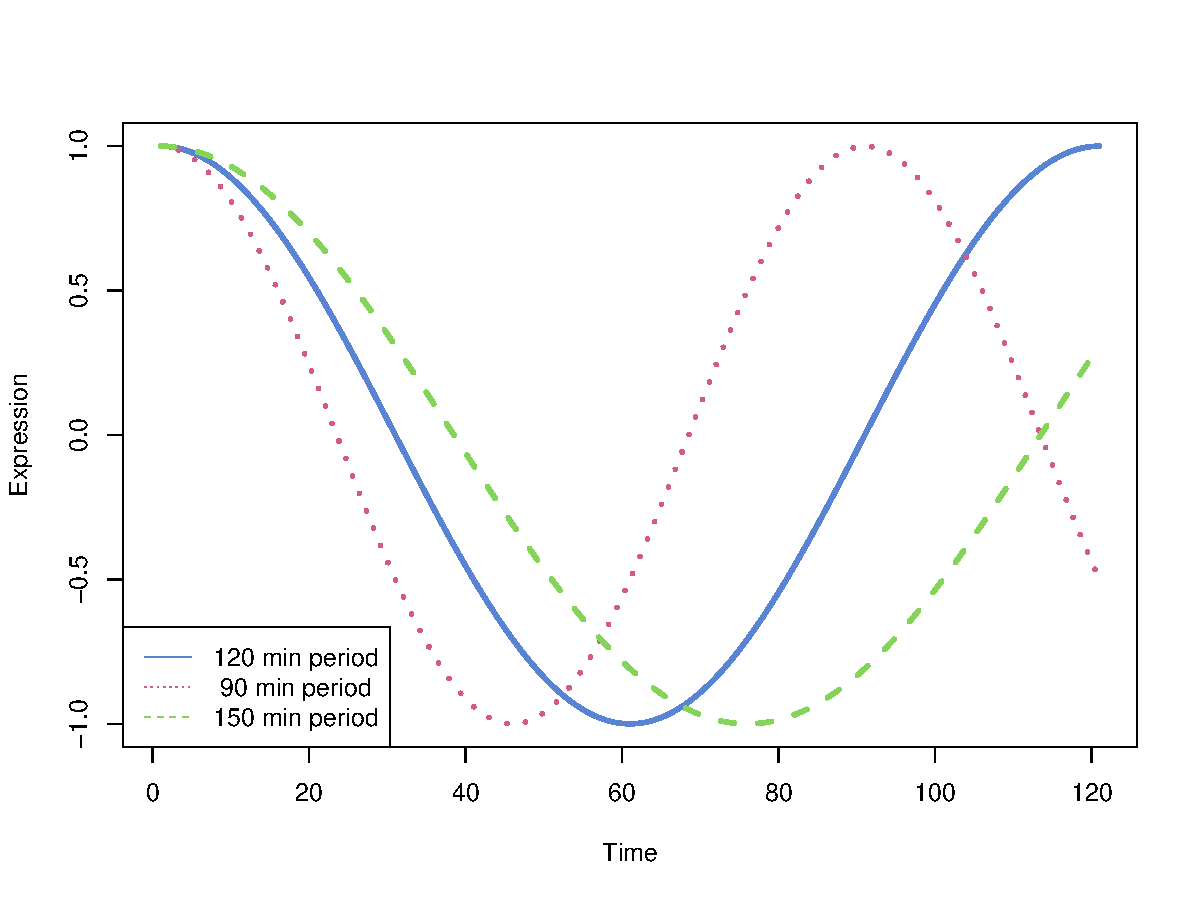
\includegraphics[width=.9\linewidth,height=.7\linewidth]{figure/lines_colored1-1} 

}



\end{knitrout}
\end{frame}

%------------------------------------------------

\begin{frame}
  \begin{center}
    {\Large Colors can dramatically impact how we perceive a graphic and what we see in the data.}
  \end{center}
\end{frame}

%------------------------------------------------

\begin{frame}
\frametitle{Why Colors?}

\bb{Importance of Color}
 \bbi
  \item Color isn't just about making your charts look pretty
  \item Color can serve as a visual cue just like the height of a bar or the position of a dot
  \item R provides a straighforward way to modify colors
 \ei
\eb

\end{frame}

%------------------------------------------------

\begin{frame}
\begin{center}
\Huge{\hilit{Naming Colors}}
\end{center}
\end{frame}

%------------------------------------------------

\begin{frame}
\frametitle{Naming colors}

\bb{Specifying colors}
There are various ways to specify colors in R
 \bi
  \item by using the color's name (in English): e.g. {\hilit \code{"turquoise"}}
  \item by using a hexadecimal string: {\hilit \code{"\#FFAA00"}} 
  \item by using standard color space functions: e.g. {\hilit \code{rgb()}}
 \ei
\eb

\end{frame}

%------------------------------------------------

\begin{frame}[fragile]
\frametitle{Function \code{colors()}}

The easiest way to specify a color in R is simply to use the color's name. The R function {\hilit \code{colors()}} provides the names of 657 available colors
\begin{knitrout}\scriptsize
\definecolor{shadecolor}{rgb}{0.969, 0.969, 0.969}\color{fgcolor}\begin{kframe}
\begin{alltt}
\hlcom{# first 30 colors}
\hlkwd{colors}\hlstd{()[}\hlnum{1}\hlopt{:}\hlnum{30}\hlstd{]}
\end{alltt}
\begin{verbatim}
##  [1] "white"          "aliceblue"      "antiquewhite"   "antiquewhite1" 
##  [5] "antiquewhite2"  "antiquewhite3"  "antiquewhite4"  "aquamarine"    
##  [9] "aquamarine1"    "aquamarine2"    "aquamarine3"    "aquamarine4"   
## [13] "azure"          "azure1"         "azure2"         "azure3"        
## [17] "azure4"         "beige"          "bisque"         "bisque1"       
## [21] "bisque2"        "bisque3"        "bisque4"        "black"         
## [25] "blanchedalmond" "blue"           "blue1"          "blue2"         
## [29] "blue3"          "blue4"
\end{verbatim}
\end{kframe}
\end{knitrout}

\end{frame}

%------------------------------------------------

\begin{frame}[fragile]
\frametitle{Function \code{colors()}}

\begin{knitrout}\scriptsize
\definecolor{shadecolor}{rgb}{0.969, 0.969, 0.969}\color{fgcolor}\begin{kframe}
\begin{alltt}
\hlcom{# first 10 colors()}
\hlkwd{pie}\hlstd{(}\hlkwd{rep}\hlstd{(}\hlnum{1}\hlstd{,} \hlnum{10}\hlstd{),} \hlkwc{col} \hlstd{=} \hlkwd{colors}\hlstd{()[}\hlnum{1}\hlopt{:}\hlnum{10}\hlstd{],} \hlkwc{labels} \hlstd{=} \hlkwd{colors}\hlstd{()[}\hlnum{1}\hlopt{:}\hlnum{10}\hlstd{])}
\end{alltt}
\end{kframe}

{\centering 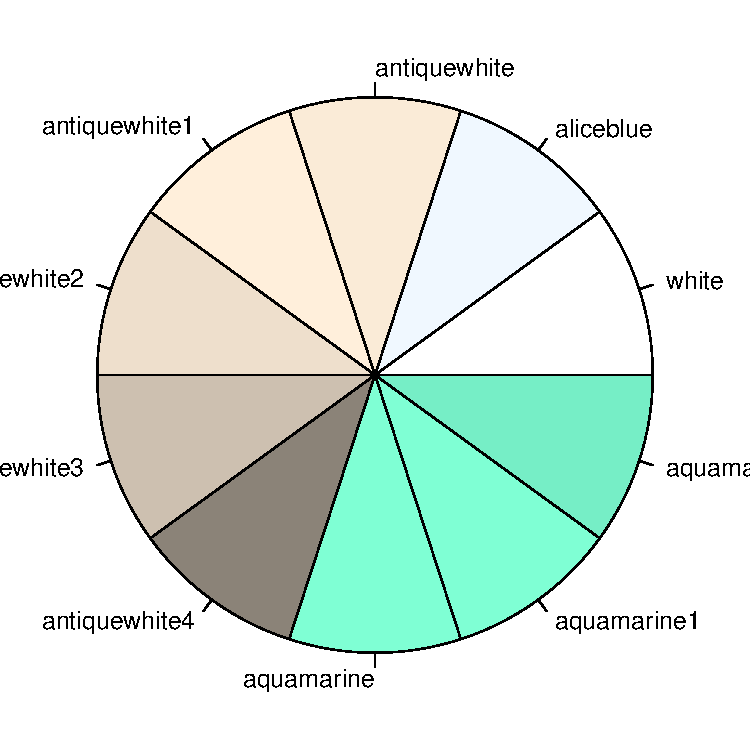
\includegraphics[width=.4\linewidth,height=.4\linewidth]{figure/unnamed-chunk-1-1} 

}



\end{knitrout}

\end{frame}

%------------------------------------------------

\begin{frame}[fragile]
\frametitle{More \code{colors()}}

Use \code{grep()} to get colors of a given name
\begin{knitrout}\scriptsize
\definecolor{shadecolor}{rgb}{0.969, 0.969, 0.969}\color{fgcolor}\begin{kframe}
\begin{alltt}
\hlcom{# orangey colors}
\hlkwd{colors}\hlstd{()[}\hlkwd{grep}\hlstd{(}\hlstr{"orange"}\hlstd{,} \hlkwd{colors}\hlstd{())]}
\end{alltt}
\begin{verbatim}
##  [1] "darkorange"  "darkorange1" "darkorange2" "darkorange3" "darkorange4"
##  [6] "orange"      "orange1"     "orange2"     "orange3"     "orange4"    
## [11] "orangered"   "orangered1"  "orangered2"  "orangered3"  "orangered4"
\end{verbatim}
\end{kframe}
\end{knitrout}

\end{frame}

%------------------------------------------------

\begin{frame}[fragile]
\frametitle{Orangey \code{colors()}}

\begin{knitrout}\scriptsize
\definecolor{shadecolor}{rgb}{0.969, 0.969, 0.969}\color{fgcolor}\begin{kframe}
\begin{alltt}
\hlcom{# orangey colors()}
\hlstd{oranges} \hlkwb{<-} \hlkwd{colors}\hlstd{()[}\hlkwd{grep}\hlstd{(}\hlstr{"orange"}\hlstd{,} \hlkwd{colors}\hlstd{())]}
\hlkwd{pie}\hlstd{(}\hlkwd{rep}\hlstd{(}\hlnum{1}\hlstd{,} \hlkwd{length}\hlstd{(oranges)),} \hlkwc{col} \hlstd{= oranges,} \hlkwc{labels} \hlstd{= oranges)}
\end{alltt}
\end{kframe}

{\centering 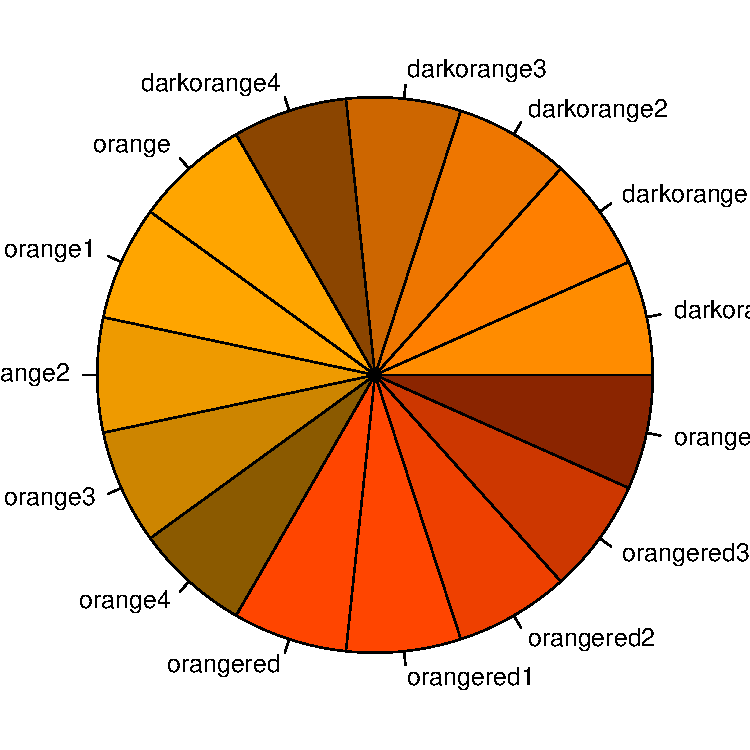
\includegraphics[width=.4\linewidth,height=.4\linewidth]{figure/unnamed-chunk-2-1} 

}



\end{knitrout}

\end{frame}

%------------------------------------------------



%------------------------------------------------

\begin{frame}[fragile]

\begin{knitrout}\tiny
\definecolor{shadecolor}{rgb}{0.969, 0.969, 0.969}\color{fgcolor}

{\centering 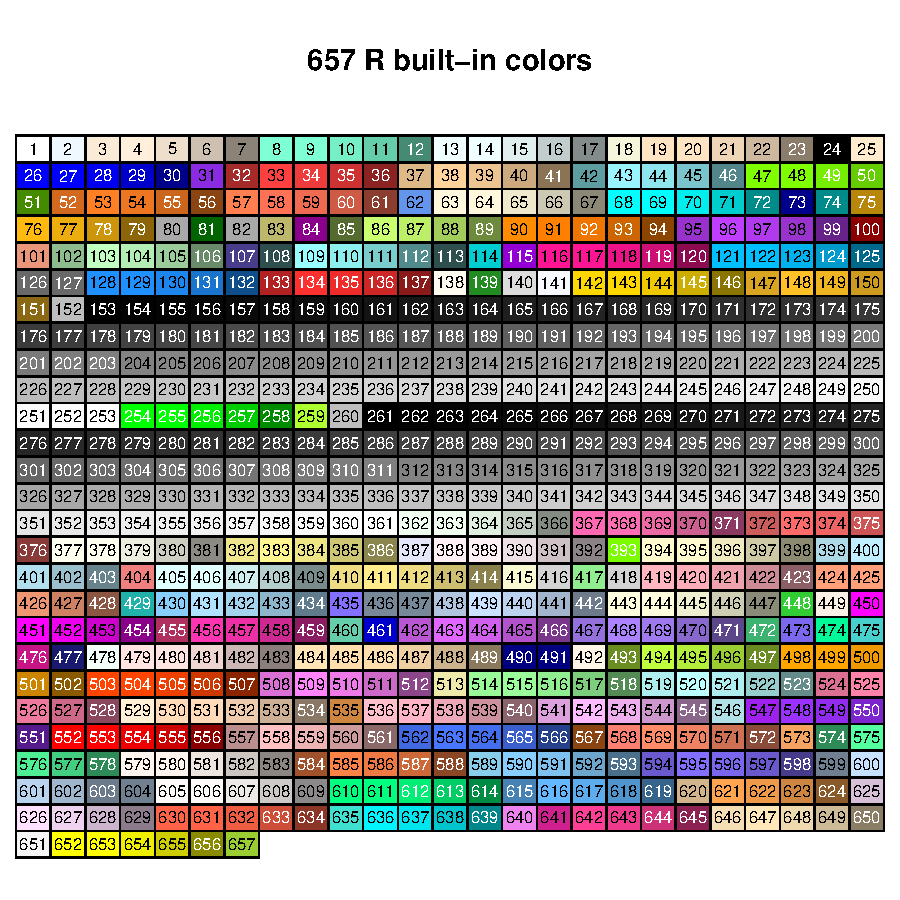
\includegraphics[width=.85\linewidth,height=.85\linewidth]{figure/R_colors-1} 

}



\end{knitrout}

\end{frame}

%------------------------------------------------

\begin{frame}[fragile]
\begin{knitrout}\tiny
\definecolor{shadecolor}{rgb}{0.969, 0.969, 0.969}\color{fgcolor}\begin{kframe}
\begin{alltt}
\hlcom{# Code by Earl F. Glynn}
\hlstd{SetTextContrastColor} \hlkwb{<-} \hlkwa{function}\hlstd{(}\hlkwc{color}\hlstd{) \{}
  \hlkwd{ifelse}\hlstd{(} \hlkwd{mean}\hlstd{(}\hlkwd{col2rgb}\hlstd{(color))} \hlopt{>} \hlnum{127}\hlstd{,} \hlstr{"black"}\hlstd{,} \hlstr{"white"}\hlstd{)}
\hlstd{\}}
\hlstd{TextContrastColor} \hlkwb{<-} \hlkwd{unlist}\hlstd{(}\hlkwd{lapply}\hlstd{(}\hlkwd{colors}\hlstd{(), SetTextContrastColor))}

\hlstd{colCount} \hlkwb{<-} \hlnum{25} \hlcom{# number per row}
\hlstd{rowCount} \hlkwb{<-} \hlnum{27}

\hlstd{op} \hlkwb{<-} \hlkwd{par}\hlstd{(}\hlkwc{mar} \hlstd{=} \hlkwd{c}\hlstd{(}\hlnum{0}\hlstd{,} \hlnum{0}\hlstd{,} \hlnum{4}\hlstd{,} \hlnum{0}\hlstd{))}
\hlkwd{plot}\hlstd{(}\hlkwd{c}\hlstd{(}\hlnum{1}\hlstd{, colCount),} \hlkwd{c}\hlstd{(}\hlnum{0}\hlstd{, rowCount),} \hlkwc{type} \hlstd{=} \hlstr{"n"}\hlstd{,} \hlkwc{axes}\hlstd{=}\hlnum{FALSE}\hlstd{,}
     \hlkwc{ylab} \hlstd{=} \hlstr{""}\hlstd{,} \hlkwc{xlab} \hlstd{=} \hlstr{""}\hlstd{,} \hlkwc{ylim} \hlstd{=} \hlkwd{c}\hlstd{(rowCount,} \hlnum{0}\hlstd{))}
\hlkwd{title}\hlstd{(}\hlstr{"657 R built-in colors"}\hlstd{)}
\hlkwa{for} \hlstd{(j} \hlkwa{in} \hlnum{0}\hlopt{:}\hlstd{(rowCount}\hlopt{-}\hlnum{1}\hlstd{))}
\hlstd{\{}
  \hlstd{base} \hlkwb{<-} \hlstd{j} \hlopt{*} \hlstd{colCount}
  \hlstd{remaining} \hlkwb{<-} \hlkwd{length}\hlstd{(}\hlkwd{colors}\hlstd{())} \hlopt{-} \hlstd{base}
  \hlstd{RowSize} \hlkwb{<-} \hlkwd{ifelse}\hlstd{(remaining} \hlopt{<} \hlstd{colCount, remaining, colCount)}
  \hlkwd{rect}\hlstd{((}\hlnum{1}\hlopt{:}\hlstd{RowSize)}\hlopt{-}\hlnum{0.5}\hlstd{, j}\hlopt{-}\hlnum{0.5}\hlstd{, (}\hlnum{1}\hlopt{:}\hlstd{RowSize)}\hlopt{+}\hlnum{0.5}\hlstd{, j}\hlopt{+}\hlnum{0.5}\hlstd{,}
       \hlkwc{border} \hlstd{=} \hlstr{"black"}\hlstd{,} \hlkwc{col} \hlstd{=} \hlkwd{colors}\hlstd{()[base} \hlopt{+} \hlstd{(}\hlnum{1}\hlopt{:}\hlstd{RowSize)])}
  \hlkwd{text}\hlstd{((}\hlnum{1}\hlopt{:}\hlstd{RowSize), j,} \hlkwd{paste}\hlstd{(base} \hlopt{+} \hlstd{(}\hlnum{1}\hlopt{:}\hlstd{RowSize)),} \hlkwc{cex} \hlstd{=} \hlnum{0.7}\hlstd{,}
       \hlkwc{col} \hlstd{= TextContrastColor[base} \hlopt{+} \hlstd{(}\hlnum{1}\hlopt{:}\hlstd{RowSize)])}
\hlstd{\}}
\hlkwd{par}\hlstd{(op)}
\end{alltt}
\end{kframe}
\end{knitrout}

{\scriptsize \url{http://research.stowers-institute.org/efg/R/Color/Chart/index.htm}}

\end{frame}

%------------------------------------------------

\begin{frame}[fragile]
\frametitle{Gray \code{colors()}}

Note that there is a wide range of gray (grey) colors:
\begin{knitrout}\scriptsize
\definecolor{shadecolor}{rgb}{0.969, 0.969, 0.969}\color{fgcolor}\begin{kframe}
\begin{alltt}
\hlcom{# gray and grey colors}
\hlstd{grays} \hlkwb{<-} \hlkwd{colors}\hlstd{()[}\hlkwd{grep}\hlstd{(}\hlstr{"gr[a|e]y"}\hlstd{,} \hlkwd{colors}\hlstd{())]}
\hlkwd{length}\hlstd{(grays)}
\end{alltt}
\begin{verbatim}
## [1] 224
\end{verbatim}
\begin{alltt}
\hlkwd{head}\hlstd{(grays,} \hlnum{10}\hlstd{)}
\end{alltt}
\begin{verbatim}
##  [1] "darkgray"       "darkgrey"       "darkslategray"  "darkslategray1"
##  [5] "darkslategray2" "darkslategray3" "darkslategray4" "darkslategrey" 
##  [9] "dimgray"        "dimgrey"
\end{verbatim}
\end{kframe}
\end{knitrout}

\end{frame}

%------------------------------------------------

\begin{frame}[fragile]
\frametitle{Example}
\begin{knitrout}\scriptsize
\definecolor{shadecolor}{rgb}{0.969, 0.969, 0.969}\color{fgcolor}\begin{kframe}
\begin{alltt}
\hlcom{# color argument 'col'}
\hlkwd{plot}\hlstd{(mtcars}\hlopt{$}\hlstd{mpg, mtcars}\hlopt{$}\hlstd{hp,} \hlkwc{pch} \hlstd{=} \hlnum{19}\hlstd{,} \hlkwc{col} \hlstd{=} \hlstr{"blue"}\hlstd{,} \hlkwc{cex} \hlstd{=} \hlnum{1.2}\hlstd{)}
\end{alltt}
\end{kframe}

{\centering 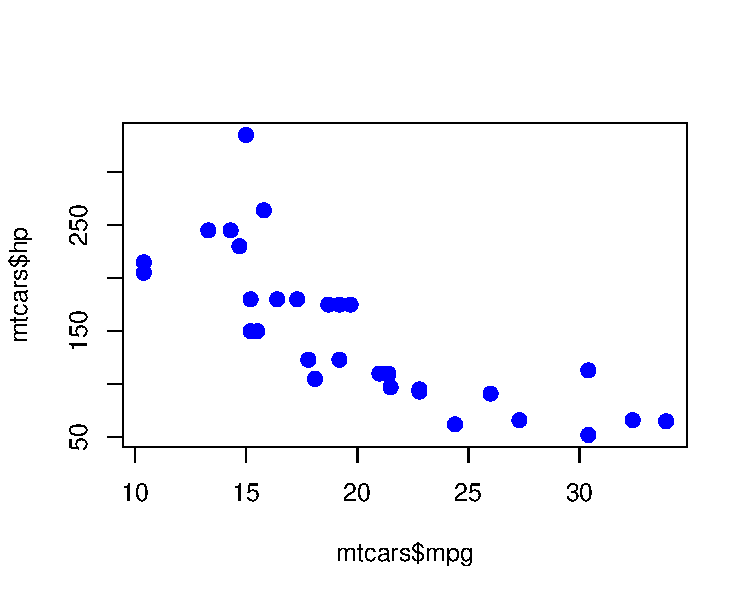
\includegraphics[width=.65\linewidth,height=.6\linewidth]{figure/unnamed-chunk-3-1} 

}



\end{knitrout}
\end{frame}

%------------------------------------------------

\begin{frame}
\begin{center}
\Huge{\hilit{RGB Color Model}}
\end{center}
\end{frame}

%------------------------------------------------

\begin{frame}
\frametitle{RGB Colors}

\bb{About RGB color}
 \bi
  \item Computers create the colors we see on a monitor by combining 3 primary colors of light: 
  \bi
    \item red
    \item green
    \item blue
  \ei
  \item This combination is known as \textbf{RGB color model}
  \item Each color light is also referred to as a \textbf{channel}
 \ei
\eb

\end{frame}

%------------------------------------------------

\begin{frame}[fragile]
\frametitle{Red-Green-Blue}

A computer screen displays a color by combining red light, green light and blue light, the so-called RGB model.

\begin{center}
\ig[width=5cm]{images/rgbcolor.jpg}
\end{center}
\end{frame}

%------------------------------------------------

\begin{frame}
\frametitle{RGB Colors}

\bb{Values of RGB colors}
 \bbi
  \item Any color you see on a monitor can be described by a series of 3 numbers (in the following order): 
  \bi
    \item a red value
    \item a green value
    \item a blue value
  \ei
  \item e.g. red=30, green=200, blue=180
 \ei
\eb

\end{frame}

%------------------------------------------------

\begin{frame}
\frametitle{RGB Colors}

\bb{Values of RGB colors}
 \bbi
  \item The amount of light in each color channel is typically described on a scale from 0 (none) to 255 (full-blast)
  \item Alternatively, scales can be provided as percent  values from 0 (none) to 1 (100\%)
 \ei
\eb

\end{frame}

%------------------------------------------------

\begin{frame}
\frametitle{RGB Colors}

Some reference colors:
\begin{center}
 \begin{tabular}{l l}
  \hline
  RGB Values & Color \\
  \hline
  \code{(255, 0, 0)} & red \\  
  \code{(0, 255, 0)} & green \\
  \code{(0, 0, 255)} & blue \\
  \code{(0, 0, 0)} & black \\
  \code{(255, 255, 255)} & white \\
  \hline
 \end{tabular}
\end{center}

The closer the three values get to 255 (100\%), the closer the resulting color gets to white
\end{frame}

%------------------------------------------------

\begin{frame}[fragile]
\frametitle{\code{rgb()} colors}

R provides the function {\hilit \code{rgb()}} to specify RGB colors
\begin{knitrout}\footnotesize
\definecolor{shadecolor}{rgb}{0.969, 0.969, 0.969}\color{fgcolor}\begin{kframe}
\begin{alltt}
\hlcom{# 0 to 1 (default scale)}
\hlkwd{rgb}\hlstd{(}\hlkwc{red} \hlstd{=} \hlnum{1}\hlstd{,} \hlkwc{green} \hlstd{=} \hlnum{0}\hlstd{,} \hlkwc{blue} \hlstd{=} \hlnum{0}\hlstd{)}
\end{alltt}
\begin{verbatim}
## [1] "#FF0000"
\end{verbatim}
\begin{alltt}
\hlcom{# 0 to 255}
\hlkwd{rgb}\hlstd{(}\hlkwc{red} \hlstd{=} \hlnum{255}\hlstd{,} \hlkwc{green} \hlstd{=} \hlnum{0}\hlstd{,} \hlkwc{blue} \hlstd{=} \hlnum{0}\hlstd{,} \hlkwc{maxColorValue} \hlstd{=} \hlnum{255}\hlstd{)}
\end{alltt}
\begin{verbatim}
## [1] "#FF0000"
\end{verbatim}
\end{kframe}
\end{knitrout}

\end{frame}

%------------------------------------------------

\begin{frame}[fragile]
\frametitle{Example}
\begin{knitrout}\scriptsize
\definecolor{shadecolor}{rgb}{0.969, 0.969, 0.969}\color{fgcolor}\begin{kframe}
\begin{alltt}
\hlcom{# color argument 'col'}
\hlkwd{plot}\hlstd{(mtcars}\hlopt{$}\hlstd{mpg, mtcars}\hlopt{$}\hlstd{hp,} \hlkwc{pch} \hlstd{=} \hlnum{19}\hlstd{,} \hlkwc{cex} \hlstd{=} \hlnum{1.2}\hlstd{,}
     \hlkwc{col} \hlstd{=} \hlkwd{rgb}\hlstd{(}\hlnum{255}\hlstd{,} \hlnum{0}\hlstd{,} \hlnum{0}\hlstd{,} \hlkwc{max} \hlstd{=} \hlnum{255}\hlstd{))}
\end{alltt}
\end{kframe}

{\centering 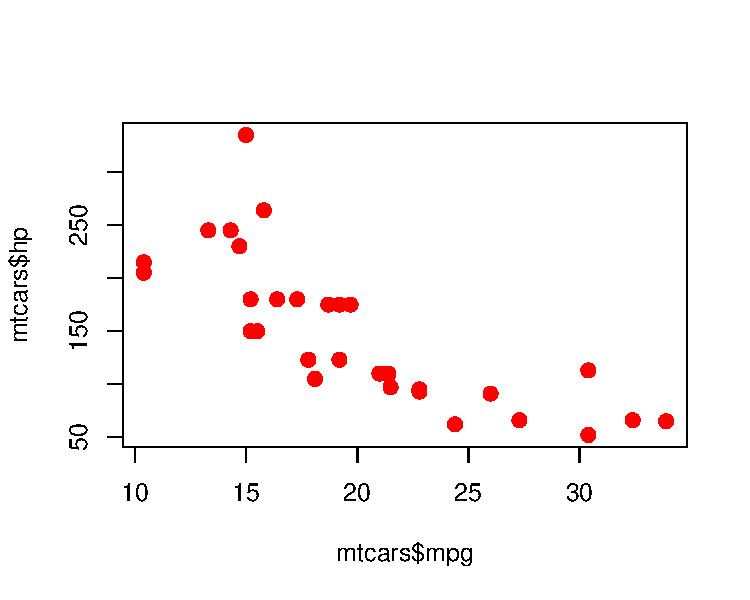
\includegraphics[width=.65\linewidth,height=.5\linewidth]{figure/unnamed-chunk-5-1} 

}



\end{knitrout}
\end{frame}

%------------------------------------------------

\begin{frame}
\begin{center}
\Huge{\hilit{Colors in Hexadecimal Notation}}
\end{center}
\end{frame}

%------------------------------------------------

\begin{frame}
\frametitle{Hex Colors}

\begin{center}
Storing RGB colors in decimal notation would require 9 digits:
\bigskip

{\large \code{255|255|255}}
\pause

\bigskip
In order to have a more efficient storage system, computers use \textbf{hexadecimal digits}
\end{center}

\end{frame}

%------------------------------------------------

\begin{frame}
\frametitle{Hex Colors}

\bb{Colors in hexadecimal notation}
A color can also be specified as a string beginning with a hash symbol \code{"\#"} and followed by six hexadecimal digits
 \bi
  \item \code{"\#FF0000"} (red)
  \item \code{"\#00FF00"} (green)
  \item \code{"\#0000FF"} (blue)
  \item \code{"\#FF6347"} (tomato)
 \ei
\eb

This is actually the output format of \code{rgb()}
\end{frame}

%------------------------------------------------

\begin{frame}[fragile]
\frametitle{Example}
\begin{knitrout}\scriptsize
\definecolor{shadecolor}{rgb}{0.969, 0.969, 0.969}\color{fgcolor}\begin{kframe}
\begin{alltt}
\hlcom{# color argument 'col'}
\hlkwd{plot}\hlstd{(mtcars}\hlopt{$}\hlstd{mpg, mtcars}\hlopt{$}\hlstd{hp,} \hlkwc{pch} \hlstd{=} \hlnum{19}\hlstd{,} \hlkwc{cex} \hlstd{=} \hlnum{1.2}\hlstd{,}
     \hlkwc{col} \hlstd{=} \hlstr{"#559944"}\hlstd{)}
\end{alltt}
\end{kframe}

{\centering 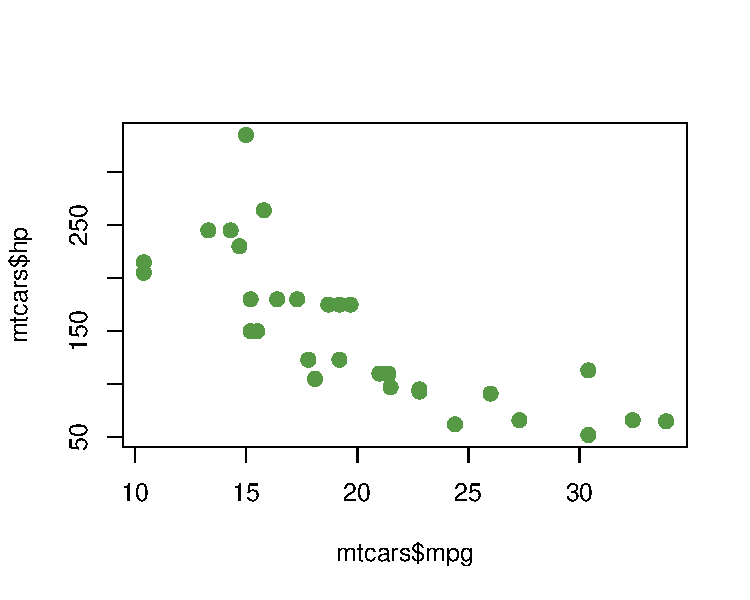
\includegraphics[width=.65\linewidth,height=.6\linewidth]{figure/unnamed-chunk-6-1} 

}



\end{knitrout}
\end{frame}

%------------------------------------------------

\begin{frame}
\frametitle{Hexadecimal code}

\begin{center}
Hexadecimal: numeral system with base 16, or \textit{hex}

\bigskip
\ig[width=10cm]{images/hex_digits.pdf}
\end{center}

\end{frame}

%------------------------------------------------

\begin{frame}
\frametitle{Hexadecimal code}

\bb{R uses the hexadecimal system to name colors}
 \bi
  \item The hexadecimal representation uses 16 different symbols
  \item The 16 symbols are all 10 digits (0-9) and 6 first letters (A-F)
  \item The digits 0-9 represent values zero to nine
  \item The letters A, B, C, D, E, F (or a, b, c, d, e, f) represent values ten to fifteen
 \ei
\eb

\end{frame}

%------------------------------------------------

\begin{frame}[fragile]
\frametitle{Hexadecimal Notation}

Decimal and Hexadecimal
\begin{knitrout}\scriptsize
\definecolor{shadecolor}{rgb}{0.969, 0.969, 0.969}\color{fgcolor}\begin{kframe}
\begin{verbatim}
##             1 2 3 4 5 6 7 8 9 10 11 12 13 14 15 16
## decimal     0 1 2 3 4 5 6 7 8  9 10 11 12 13 14 15
## hexadecimal 0 1 2 3 4 5 6 7 8  9  A  B  C  D  E  F
\end{verbatim}
\end{kframe}
\end{knitrout}

{\lit Two hexadecimal digits together can make $16 \times 16 = 256$ different values (from 0 to 255)

\bigskip
Six hexadecimal digits together can make $16^6 = 16,777,216$ different values.}
\end{frame}

%------------------------------------------------

\begin{frame}
\frametitle{Hexadecimal code}

\bb{Hexadecimal color: \code{\#975015}}
 \bi
  \item {\hilit \code{\#}} declares that this ``is a hex number''
  \item The other six are really three sets of pairs
  \item Each pair controls one primary additive color
  \item The first pair corresponds to red
  \item The second pair corresponds to green
  \item The last pair corresponds to blue
 \ei
\eb

\end{frame}

%------------------------------------------------

\begin{frame}[fragile]
\begin{center}
\ig[width=8cm]{images/hexcolor.pdf}
\end{center}
There are 256 possible shades each of red, green, and blue
\end{frame}

%------------------------------------------------

\begin{frame}[fragile]
\frametitle{RGB Hexadecimal Notation}

\begin{knitrout}\scriptsize
\definecolor{shadecolor}{rgb}{0.969, 0.969, 0.969}\color{fgcolor}

{\centering 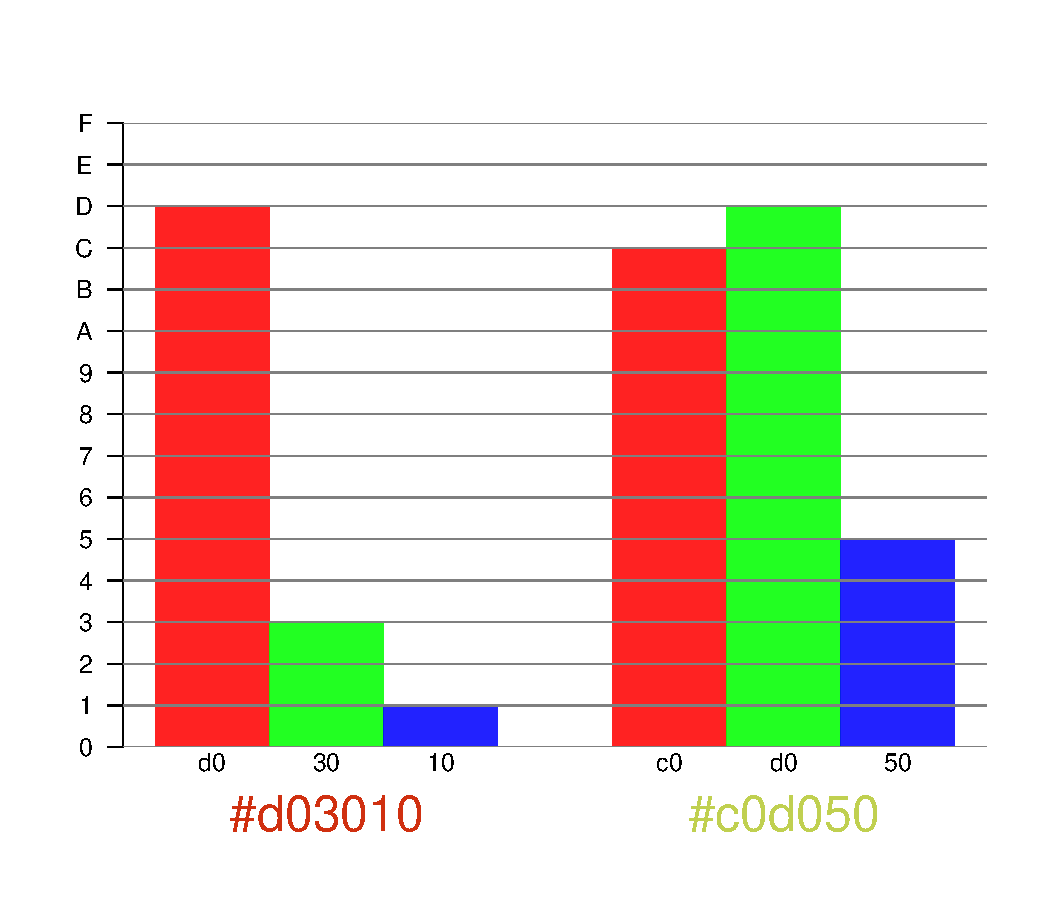
\includegraphics[width=.7\linewidth,height=.6\linewidth]{figure/unnamed-chunk-8-1} 

}



\end{knitrout}

\end{frame}

%------------------------------------------------

\begin{frame}
\frametitle{Hexadecimal code}

\bb{Hexadecimal digits}
 \bi
  \item \textbf{0} is the smallest representation of a color (absence of color)
  \item \textbf{F} is 15 times the intensity of color 0
  \item \textbf{00} is equal to zero hue
  \item \textbf{FF} is equal to a pure color
  \item \textbf{\#000000} black
  \item \textbf{\#FFFFFF} white
  \item equal digits produce a shade of gray
 \ei
\eb

\end{frame}

%------------------------------------------------

\begin{frame}[fragile]
\frametitle{RGB and Hex}
\begin{center}
\ig[width=8cm]{images/hexrgb.pdf}
\end{center}
\end{frame}

%------------------------------------------------

\begin{frame}
\frametitle{RGB Cube Representation}
\begin{center}
\ig[width=6cm]{images/rgbcube.png}

{\scriptsize \url{http://drmoron.org/is-black-a-color/}}
\end{center}

\end{frame}

%------------------------------------------------

\begin{frame}
\frametitle{Your turn}

{\large Orange in hex-code is:}
\bbi
  \item[A)] \code{\#FFA500}
  \item[B)] \code{\#3EDCD9}
  \item[C)] \code{\#A500FF}
  \item[D)] \code{\#E88472}
\ei

\end{frame}

%------------------------------------------------

\begin{frame}
\frametitle{Your turn}

{\large What color is RGB: 89, 132, 212}
\bbi
  \item[A)] {\hilit Orange}
  \item[B)] {\mdlit Blue}
  \item[C)] Black
  \item[D)] {\lit Yellow}
\ei

\end{frame}

%------------------------------------------------

\begin{frame}
\frametitle{RGB Inconvenience}

\bb{RGB drawbacks}
 \bi
  \item The RGB color model is the most commonly used
  \item However, specifying RGB colors in not intuitive
  \item It is no straightforward how to make a color stronger, darker or lighter with RGB values
  \item It is also hard to ``read'' RGB values (and being able to identify the corresponding hue)
 \ei
\eb

\end{frame}

%------------------------------------------------

\begin{frame}
\frametitle{Cylindrical-coordinate Representations}

\bb{Cylindrical Models}
 \bi
  \item An alternative to RGB values is the \textbf{HSV} model
  \item HSV: Hue (color), Saturation, Value
  \item HSV rearranges the geometry of RGB following cyclindrical coordinates
 \ei
\eb

\end{frame}

%------------------------------------------------

\begin{frame}
\frametitle{HSV representation}
\begin{center}
\ig[width=5cm]{images/hsvcone.png}
\end{center}
\end{frame}

%------------------------------------------------

\begin{frame}
\frametitle{Cylindrical-coordinate Representations}

\bb{HSV Models}
 \bi
  \item Hue values are measured in degrees around the circle
  \bi
    \item Red at 0 degrees
    \item Green at 120$^\circ$
    \item Blue at 240$^\circ$
    \item other colors in between
  \ei
  \item Saturation is a percentage value from 0 (gray) to 1 (full blast)
  \item Value is also a percentage value from 0 (darkest) to 1 (lightest)
 \ei
\eb

\end{frame}

%------------------------------------------------

\begin{frame}
\frametitle{Function \code{hsv()}}

R provides the function {\hilit \code{hsv()}} which takes an
HSV triplet
\begin{knitrout}\footnotesize
\definecolor{shadecolor}{rgb}{0.969, 0.969, 0.969}\color{fgcolor}\begin{kframe}
\begin{alltt}
\hlkwd{hsv}\hlstd{(}\hlkwc{h} \hlstd{=} \hlnum{1}\hlstd{,} \hlkwc{s} \hlstd{=} \hlnum{0.8}\hlstd{,} \hlkwc{v} \hlstd{=} \hlnum{0.9}\hlstd{)}
\end{alltt}
\end{kframe}
\end{knitrout}

\bigskip

Note that the Hue value ranges from 0 (0 degrees) to 1 (360 degrees)

\end{frame}

%------------------------------------------------

\begin{frame}[fragile]
\frametitle{Example}
\begin{knitrout}\scriptsize
\definecolor{shadecolor}{rgb}{0.969, 0.969, 0.969}\color{fgcolor}\begin{kframe}
\begin{alltt}
\hlcom{# hsv color}
\hlkwd{plot}\hlstd{(mtcars}\hlopt{$}\hlstd{mpg, mtcars}\hlopt{$}\hlstd{hp,} \hlkwc{pch} \hlstd{=} \hlnum{19}\hlstd{,} \hlkwc{cex} \hlstd{=} \hlnum{1.2}\hlstd{,}
     \hlkwc{col} \hlstd{=} \hlkwd{hsv}\hlstd{(}\hlkwc{h} \hlstd{=} \hlnum{1}\hlstd{,} \hlkwc{s} \hlstd{=} \hlnum{1}\hlstd{,} \hlkwc{v} \hlstd{=} \hlnum{1}\hlstd{))}
\end{alltt}
\end{kframe}

{\centering 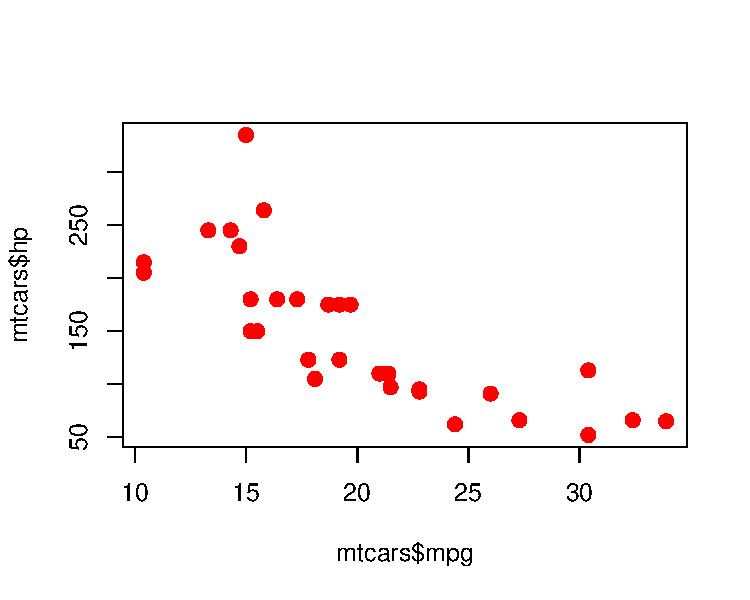
\includegraphics[width=.65\linewidth,height=.6\linewidth]{figure/unnamed-chunk-10-1} 

}



\end{knitrout}
\end{frame}

%------------------------------------------------

\begin{frame}
\frametitle{HSV}

\bb{About HSV}
 \bbi
  \item HSV is a more intuitive system
  \item HSV is also more perceptually relevant
  \item Once you select a hue, it is easy to make it stronger, darker, or lighter
 \ei
\eb

\end{frame}

%------------------------------------------------

\begin{frame}
\frametitle{Other Representations}

\bb{HCL Model}
 \bi
  \item Another model is \textbf{HCL}
  \item HCL: Hue, Chroma, Luminance
  \item Hue values are measured in degrees around the circle
  \bi
    \item Red at 0 degrees
    \item Green at 120$^\circ$
    \item Blue at 240$^\circ$
    \item other colors in between
  \ei
  \item Luminance is also a percentage value from 0 (darkest) to 100 (lightest)
  \item Chroma depends on Hue and Luminance
 \ei
\eb

\end{frame}

%------------------------------------------------

\begin{frame}[fragile]
\frametitle{Example}
\begin{knitrout}\scriptsize
\definecolor{shadecolor}{rgb}{0.969, 0.969, 0.969}\color{fgcolor}\begin{kframe}
\begin{alltt}
\hlcom{# hcl color}
\hlkwd{plot}\hlstd{(mtcars}\hlopt{$}\hlstd{mpg, mtcars}\hlopt{$}\hlstd{hp,} \hlkwc{pch} \hlstd{=} \hlnum{19}\hlstd{,} \hlkwc{cex} \hlstd{=} \hlnum{1.2}\hlstd{,}
     \hlkwc{col} \hlstd{=} \hlkwd{hcl}\hlstd{(}\hlkwc{h} \hlstd{=} \hlnum{3550}\hlstd{,} \hlkwc{c} \hlstd{=} \hlnum{75}\hlstd{,} \hlkwc{l} \hlstd{=} \hlnum{50}\hlstd{))}
\end{alltt}
\end{kframe}

{\centering 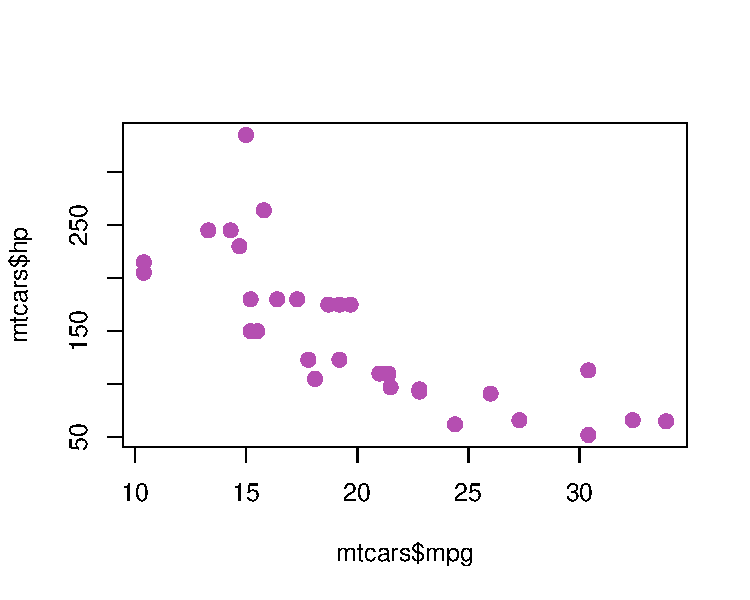
\includegraphics[width=.65\linewidth,height=.6\linewidth]{figure/unnamed-chunk-11-1} 

}



\end{knitrout}
\end{frame}

%------------------------------------------------

\begin{frame}
\frametitle{Color Space}

\bb{HSV Colors by space model}
R provides the functions \code{hsv()} and \code{hcl()}
 \bi
  \item {\hilit HSV} (Hue, Saturation, Value) triplet: \\ \code{hsv(h = 1, s = 0.8, v = 0.9)}
  \item {\hilit HCL} (Hue, Chroma, Luminance) triplet: \\ \code{hcl(h = 1, c = 35, l = 85)}
 \ei
\eb

\end{frame}

%------------------------------------------------

\begin{frame}
\frametitle{Color Space Models}

\bb{Color Model}
A \textbf{color model} is an abstract mathematical model describing the way colors can be represented as tuples of numbers, typically as three or four values or color components.
\eb

\end{frame}

%------------------------------------------------

\begin{frame}
\frametitle{About colors}

\bb{RGB Model}
The \textbf{RGB model} uses an additive color mixing with primary colors of red, green, and blue, each of which stimulates one of the three types of the eye's color receptors.
\eb

\bb{RGB usefulness}
Mixtures of light of these primary colors cover a large part of the human color space and thus produce a large part of human color experiences.
\eb

\end{frame}

%------------------------------------------------

\begin{frame}
\begin{center}
\Huge{\hilit{Semitransparent Colors}}
\end{center}
\end{frame}

%------------------------------------------------

\begin{frame}
\frametitle{Semitransparent Colors}

\bb{Color transparency}
All R colors are stored with an \textbf{alpha} transparency channel.
\bi
 \item An alpha value of 0 means fully transparent
 \item An alpha value of 1 means fully opaque
\ei
\eb

\end{frame}

%------------------------------------------------

\begin{frame}
\frametitle{Semitransparent Colors}

\bb{Alpha values}
When using any of the color space functions, transparency is indicated with the parameter {\hilit \code{alpha}}:
\bi
 \item \code{rgb(1, 0, 0, alpha = 0.5)}
 \item \code{hsv(h = 1, s = 0.8, v = 0.8, alpha = 0.5)}
 \item \code{hcl(h = 0, c = 35, l = 85, alpha = 0.5)}
\ei
\eb

\end{frame}

%------------------------------------------------

\begin{frame}
\frametitle{Semitransparent Colors}

\bb{Hex color transparency}
When using hexadecimal notation, transparency is indicated by using a hexadecimal string of \textbf{eight digits}. The last two digits indicate transparency:
\bi
 \item a hex digit \code{"00"} indicates an alpha value of 0 (fully transparent)
 \item a hex digit \code{"FF"} indicates an alpha value of 1 (fully opaque)
\ei
For example, \code{"\#FFA50080"} specifies a semitransparent orange. Note that \code{"\#FFA500"} is equivalent to \code{"\#FFA500FF"}
\eb

\end{frame}

%------------------------------------------------

\begin{frame}[fragile]
\frametitle{Hex notation with alpha channel}
\begin{center}
\ig[width=8cm]{images/hexcoloralpha.pdf}
\end{center}
\end{frame}

%------------------------------------------------

\begin{frame}
\frametitle{Transparency}

\bb{Use transparency for overlapping data}
\bi
 \item The number of lines or points on a graph can obscure other values that lie behind them.
 \item One option to present many overlapping values is to make the color values partially transparent
\ei
\eb

\end{frame}

%------------------------------------------------

\begin{frame}[fragile]
\frametitle{Example}
\begin{knitrout}\scriptsize
\definecolor{shadecolor}{rgb}{0.969, 0.969, 0.969}\color{fgcolor}\begin{kframe}
\begin{alltt}
\hlcom{# transparent color}
\hlkwd{plot}\hlstd{(iris}\hlopt{$}\hlstd{Petal.Length, iris}\hlopt{$}\hlstd{Sepal.Length,}
     \hlkwc{pch} \hlstd{=} \hlnum{19}\hlstd{,} \hlkwc{cex} \hlstd{=} \hlnum{1.2}\hlstd{,} \hlkwc{col} \hlstd{=} \hlstr{"#33994088"}\hlstd{)}
\end{alltt}
\end{kframe}

{\centering 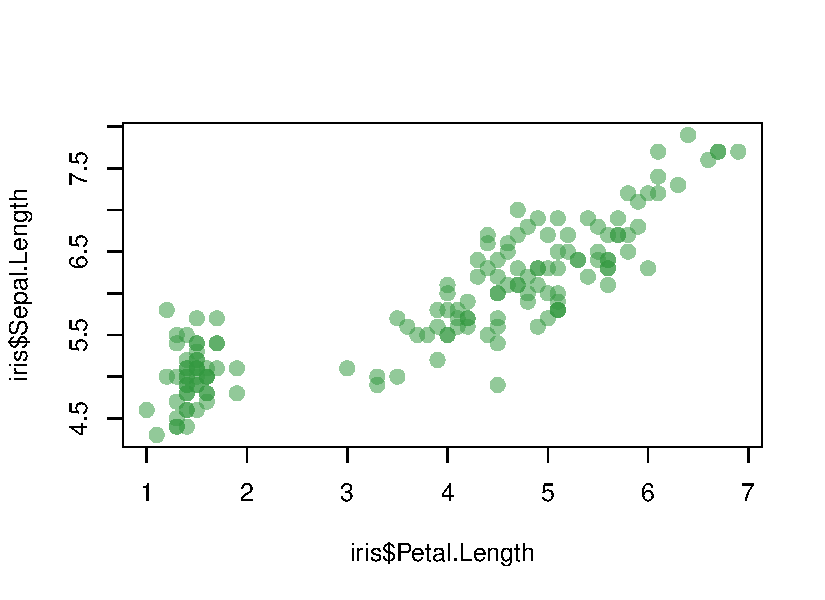
\includegraphics[width=.75\linewidth,height=.6\linewidth]{figure/unnamed-chunk-12-1} 

}



\end{knitrout}
\end{frame}

%------------------------------------------------

\begin{frame}
\frametitle{Converting Colors}

\bb{Converting colors functions}
R provides a set of functions for converting between different color spaces
\eb

\begin{center}
 \begin{tabular}{l l}
  \hline
  function & package \\
  \hline
  \code{col2rgb()} & \code{"grDevices"} \\  
  \code{hex2RGB()} & \code{"colorspace"} \\
  \code{convertColor()} & \code{"grDevices"} \\
  \hline
 \end{tabular}
\end{center}

\end{frame}

%------------------------------------------------

\begin{frame}[fragile]
\begin{knitrout}\scriptsize
\definecolor{shadecolor}{rgb}{0.969, 0.969, 0.969}\color{fgcolor}\begin{kframe}
\begin{alltt}
\hlcom{# turquoise into RGB}
\hlkwd{col2rgb}\hlstd{(}\hlstr{"turquoise"}\hlstd{)}
\end{alltt}
\begin{verbatim}
##       [,1]
## red     64
## green  224
## blue   208
\end{verbatim}
\begin{alltt}
\hlcom{# turquoise (hex) into RGB}
\hlkwd{library}\hlstd{(}\hlstr{"colorspace"}\hlstd{)}
\end{alltt}


{\ttfamily\noindent\itshape\color{messagecolor}{\#\# Loading required package: methods}}\begin{alltt}
\hlkwd{hex2RGB}\hlstd{(}\hlstr{"#40E0D0"}\hlstd{)}
\end{alltt}
\begin{verbatim}
##              R         G         B
## [1,] 0.2509804 0.8784314 0.8156863
\end{verbatim}
\begin{alltt}
\hlcom{# color 'red' sRGB into Luv}
\hlkwd{convertColor}\hlstd{(}\hlkwd{t}\hlstd{(}\hlkwd{col2rgb}\hlstd{(}\hlstr{"red"}\hlstd{)}\hlopt{/}\hlnum{255}\hlstd{),} \hlkwc{from} \hlstd{=} \hlstr{"sRGB"}\hlstd{,} \hlkwc{to} \hlstd{=} \hlstr{"Luv"}\hlstd{)}
\end{alltt}
\begin{verbatim}
##             L        u        v
## [1,] 53.48418 175.3647 37.80017
\end{verbatim}
\end{kframe}
\end{knitrout}

\end{frame}

%------------------------------------------------

\begin{frame}
\begin{center}
\Huge{\hilit{Color Palettes}}
\end{center}
\end{frame}

%------------------------------------------------

\begin{frame}
\frametitle{Color Sets}

\bb{Converting colors functions}
Usually more than one color is required within a single plot, and in such cases we need to select colors that are aesthetically pleasing  or related in some way. For this, R provides several ways to specifcy or create color schemes and palettes.
\eb

\end{frame}

%------------------------------------------------

\begin{frame}
\frametitle{R Default Palettes}

\bb{Basic Color Palettes}
R provides a set of functions to generate basic color sets.
 \bi
  \item \code{rainbow()}
  \item \code{heat.colors()}
  \item \code{topo.colors()}
  \item \code{terrain.colors()}
  \item \code{cm.colors()}
  \item \code{gray.colors()}
 \ei
\eb

\end{frame}

%------------------------------------------------

\begin{frame}[fragile]
\frametitle{Function \code{rainbow()}}

\begin{knitrout}\scriptsize
\definecolor{shadecolor}{rgb}{0.969, 0.969, 0.969}\color{fgcolor}\begin{kframe}
\begin{alltt}
\hlcom{# 8 colors rainbow}
\hlstd{n} \hlkwb{<-} \hlnum{8}
\hlkwd{pie}\hlstd{(}\hlkwd{rep}\hlstd{(}\hlnum{1}\hlstd{, n),} \hlkwc{col} \hlstd{=} \hlkwd{rainbow}\hlstd{(n))}
\end{alltt}
\end{kframe}

{\centering 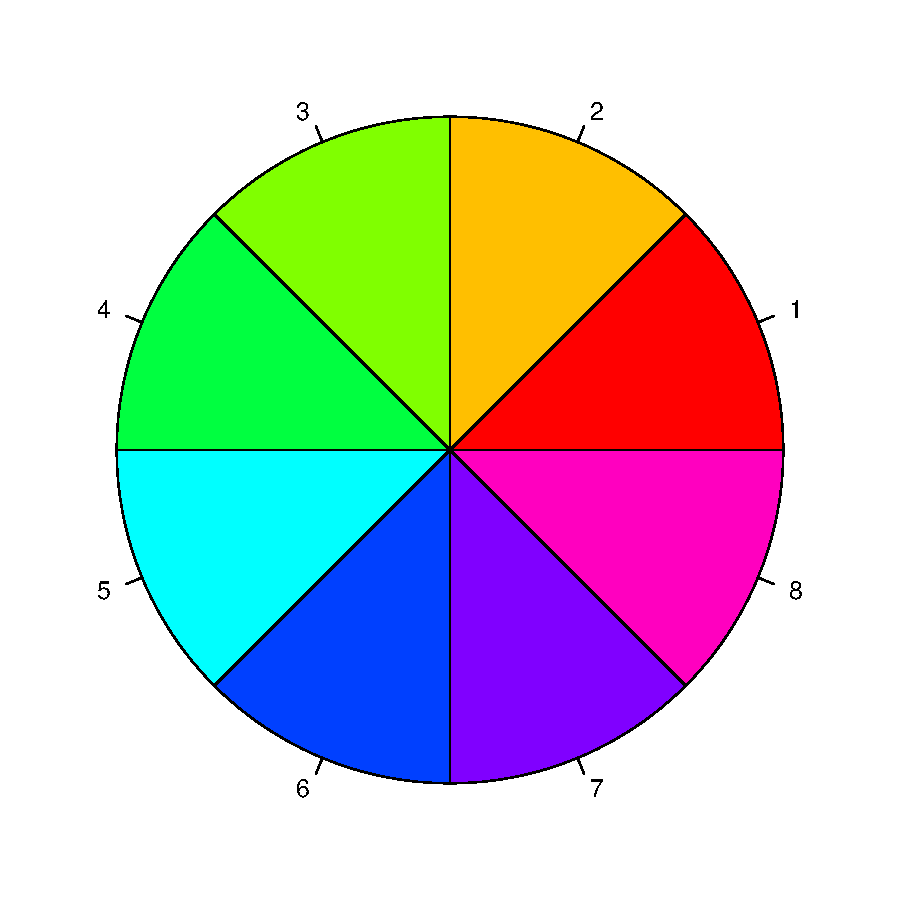
\includegraphics[width=.4\linewidth,height=.4\linewidth]{figure/rainbow-1} 

}



\end{knitrout}

\end{frame}

%------------------------------------------------

\begin{frame}[fragile]
\frametitle{Function \code{heat.colors()}}

\begin{knitrout}\scriptsize
\definecolor{shadecolor}{rgb}{0.969, 0.969, 0.969}\color{fgcolor}\begin{kframe}
\begin{alltt}
\hlcom{# heat colors (8 values)}
\hlstd{n} \hlkwb{<-} \hlnum{8}
\hlkwd{pie}\hlstd{(}\hlkwd{rep}\hlstd{(}\hlnum{1}\hlstd{, n),} \hlkwc{col} \hlstd{=} \hlkwd{heat.colors}\hlstd{(n))}
\end{alltt}
\end{kframe}

{\centering 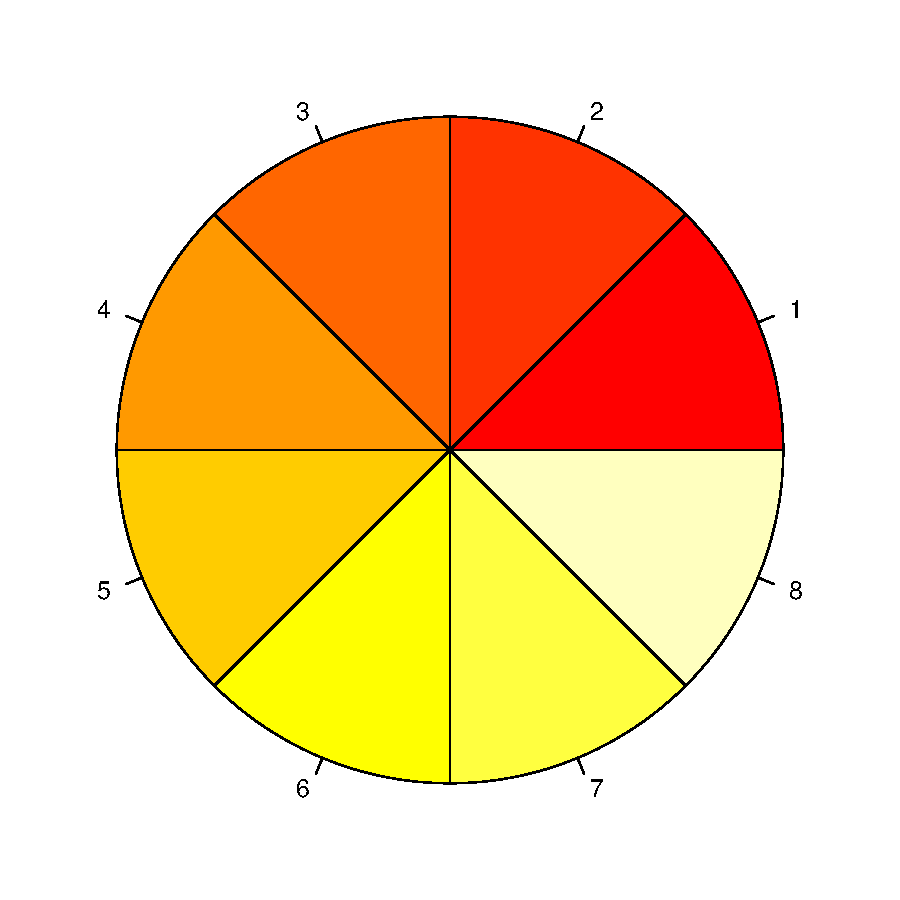
\includegraphics[width=.4\linewidth,height=.4\linewidth]{figure/heatcolors-1} 

}



\end{knitrout}

\end{frame}

%------------------------------------------------

\begin{frame}[fragile]
\frametitle{Function \code{terrain.colors()}}

\begin{knitrout}\scriptsize
\definecolor{shadecolor}{rgb}{0.969, 0.969, 0.969}\color{fgcolor}\begin{kframe}
\begin{alltt}
\hlcom{# terrain colors (8 values)}
\hlstd{n} \hlkwb{<-} \hlnum{8}
\hlkwd{pie}\hlstd{(}\hlkwd{rep}\hlstd{(}\hlnum{1}\hlstd{, n),} \hlkwc{col} \hlstd{=} \hlkwd{terrain.colors}\hlstd{(n))}
\end{alltt}
\end{kframe}

{\centering 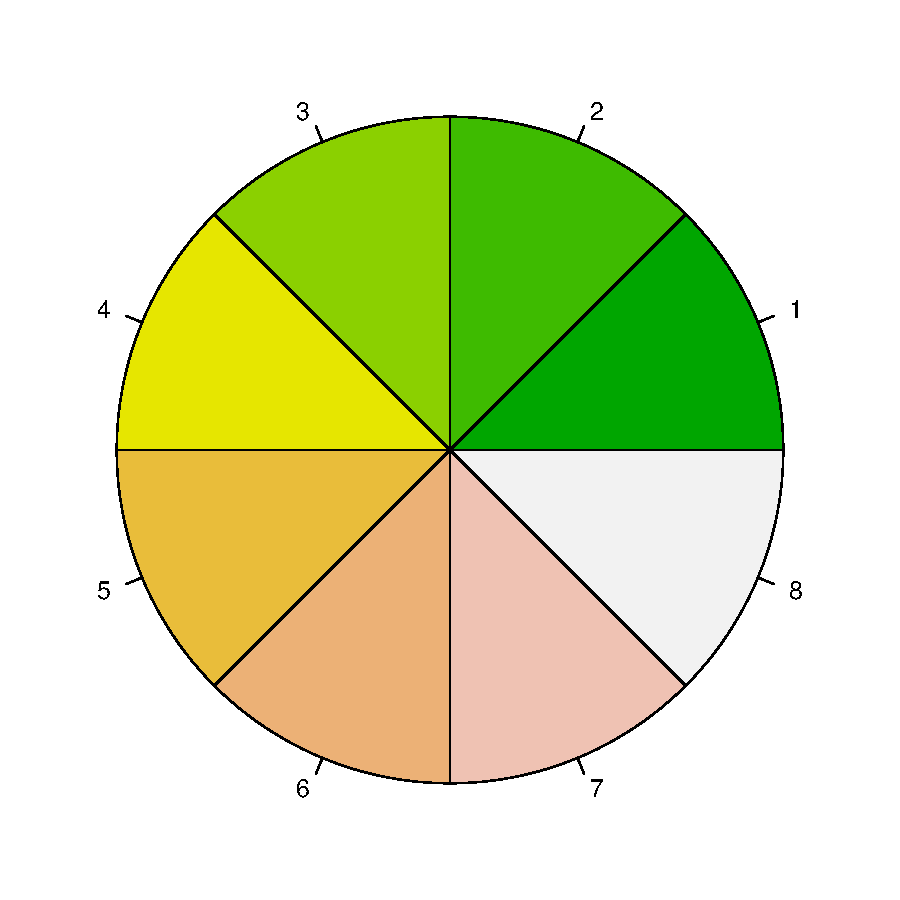
\includegraphics[width=.4\linewidth,height=.4\linewidth]{figure/terraincolors-1} 

}



\end{knitrout}

\end{frame}

%------------------------------------------------

\begin{frame}[fragile]
\frametitle{Function \code{topo.colors()}}

\begin{knitrout}\scriptsize
\definecolor{shadecolor}{rgb}{0.969, 0.969, 0.969}\color{fgcolor}\begin{kframe}
\begin{alltt}
\hlcom{# topo colors (8 values)}
\hlstd{n} \hlkwb{<-} \hlnum{8}
\hlkwd{pie}\hlstd{(}\hlkwd{rep}\hlstd{(}\hlnum{1}\hlstd{, n),} \hlkwc{col} \hlstd{=} \hlkwd{topo.colors}\hlstd{(n))}
\end{alltt}
\end{kframe}

{\centering 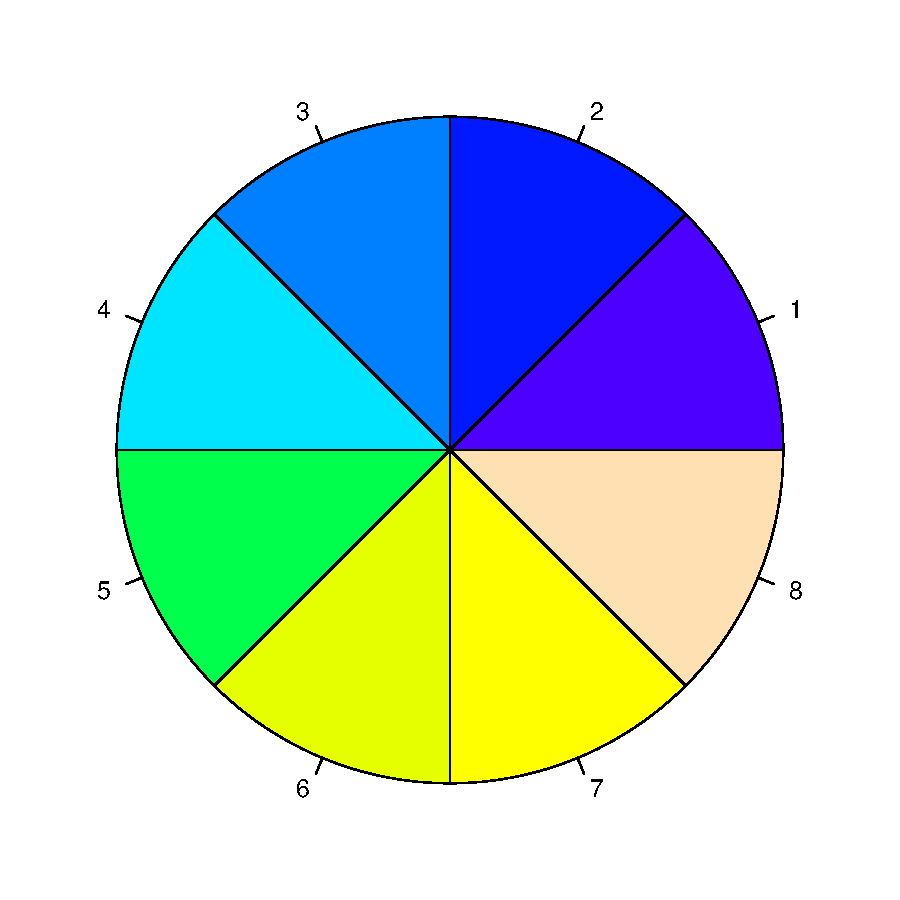
\includegraphics[width=.4\linewidth,height=.4\linewidth]{figure/topocolors-1} 

}



\end{knitrout}

\end{frame}

%------------------------------------------------

\begin{frame}[fragile]
\frametitle{Function \code{cm.colors()}}

\begin{knitrout}\scriptsize
\definecolor{shadecolor}{rgb}{0.969, 0.969, 0.969}\color{fgcolor}\begin{kframe}
\begin{alltt}
\hlcom{# cyan-magenta colors (8 values)}
\hlstd{n} \hlkwb{<-} \hlnum{8}
\hlkwd{pie}\hlstd{(}\hlkwd{rep}\hlstd{(}\hlnum{1}\hlstd{, n),} \hlkwc{col} \hlstd{=} \hlkwd{cm.colors}\hlstd{(n))}
\end{alltt}
\end{kframe}

{\centering 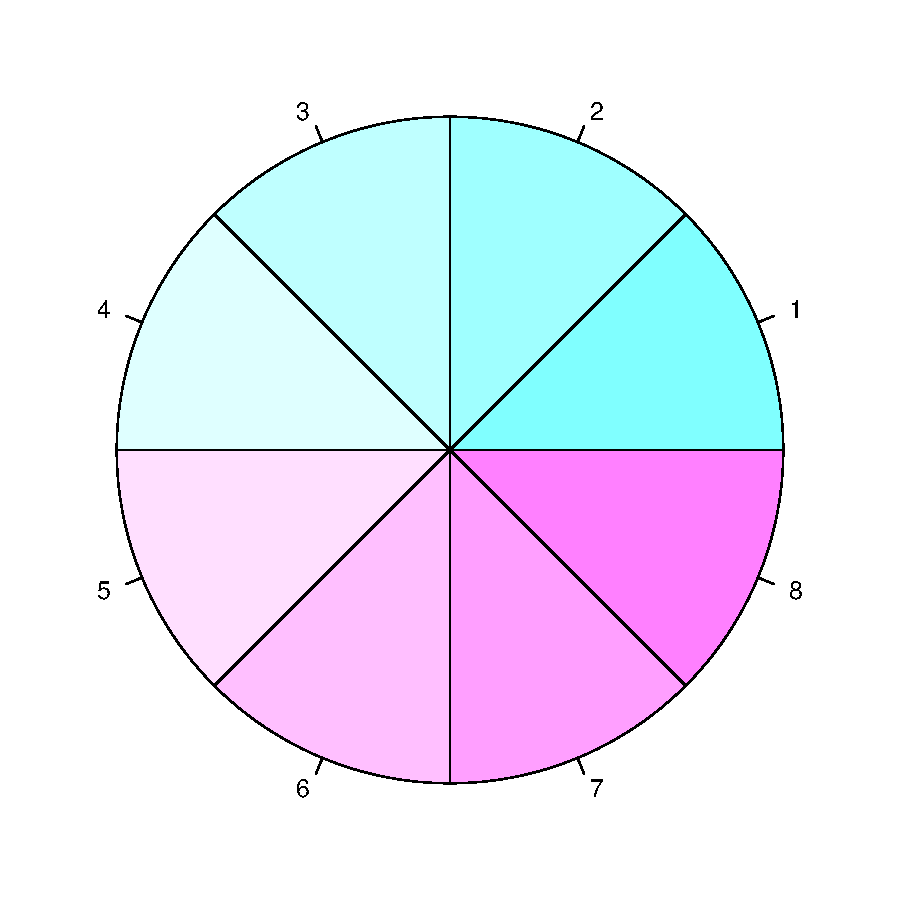
\includegraphics[width=.4\linewidth,height=.4\linewidth]{figure/cmcolors-1} 

}



\end{knitrout}

\end{frame}

%------------------------------------------------

\begin{frame}[fragile]
\frametitle{Function \code{gray.colors()}}

\begin{knitrout}\scriptsize
\definecolor{shadecolor}{rgb}{0.969, 0.969, 0.969}\color{fgcolor}\begin{kframe}
\begin{alltt}
\hlcom{# gray colors (8 values)}
\hlstd{n} \hlkwb{<-} \hlnum{8}
\hlkwd{pie}\hlstd{(}\hlkwd{rep}\hlstd{(}\hlnum{1}\hlstd{, n),} \hlkwc{col} \hlstd{=} \hlkwd{gray.colors}\hlstd{(n))}
\end{alltt}
\end{kframe}

{\centering 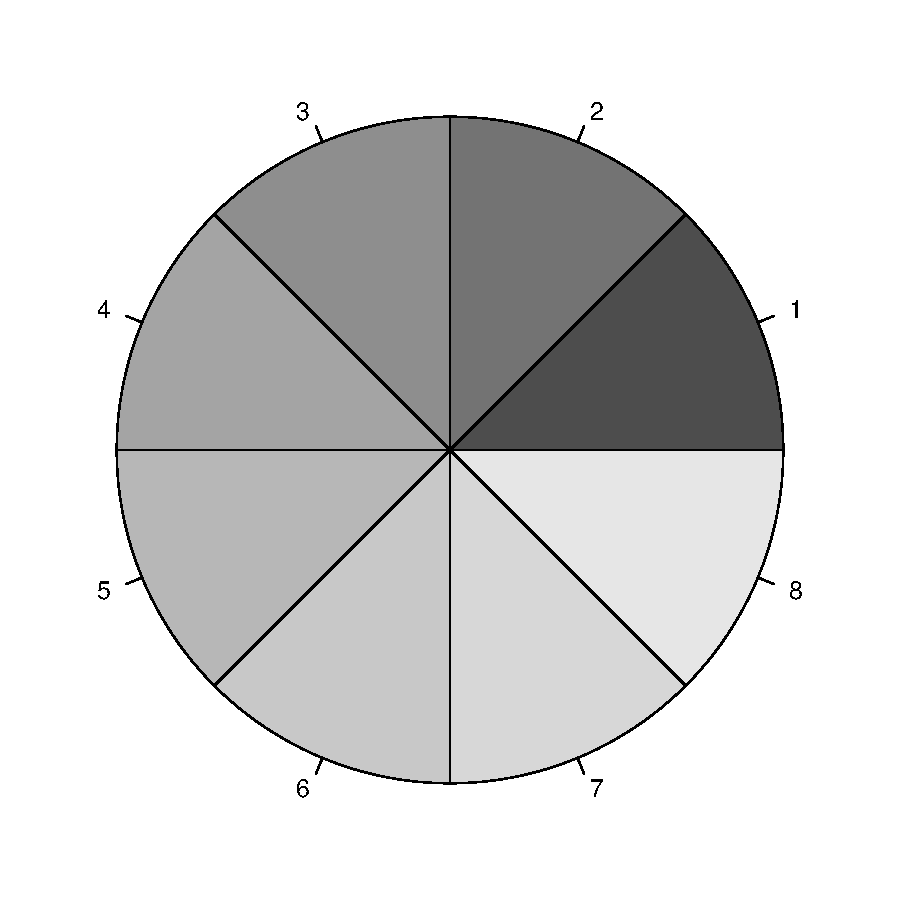
\includegraphics[width=.4\linewidth,height=.4\linewidth]{figure/garycolors-1} 

}



\end{knitrout}

\end{frame}

%------------------------------------------------

\begin{frame}[fragile]
\begin{center}
\ig[width=11cm]{images/colorbrewer.png}
\end{center}
\end{frame}

%------------------------------------------------

\begin{frame}[fragile]
\frametitle{Color Brewer}

The R package \code{"RColorBrewer"} (by Erich Neuwirth) provides nice color schemes designed by Cynthia Brewer and described at \url{http://colorbrewer2.org}

\begin{knitrout}\footnotesize
\definecolor{shadecolor}{rgb}{0.969, 0.969, 0.969}\color{fgcolor}\begin{kframe}
\begin{alltt}
\hlcom{# remember to install RColorBrewer first!}
\hlkwd{library}\hlstd{(RColorBrewer)}

\hlcom{# display available schemes }
\hlkwd{display.brewer.all}\hlstd{()}
\end{alltt}
\end{kframe}
\end{knitrout}

\end{frame}

%------------------------------------------------

\begin{frame}[fragile]
\frametitle{R Color Brewer Schemes}
\begin{knitrout}\scriptsize
\definecolor{shadecolor}{rgb}{0.969, 0.969, 0.969}\color{fgcolor}

{\centering 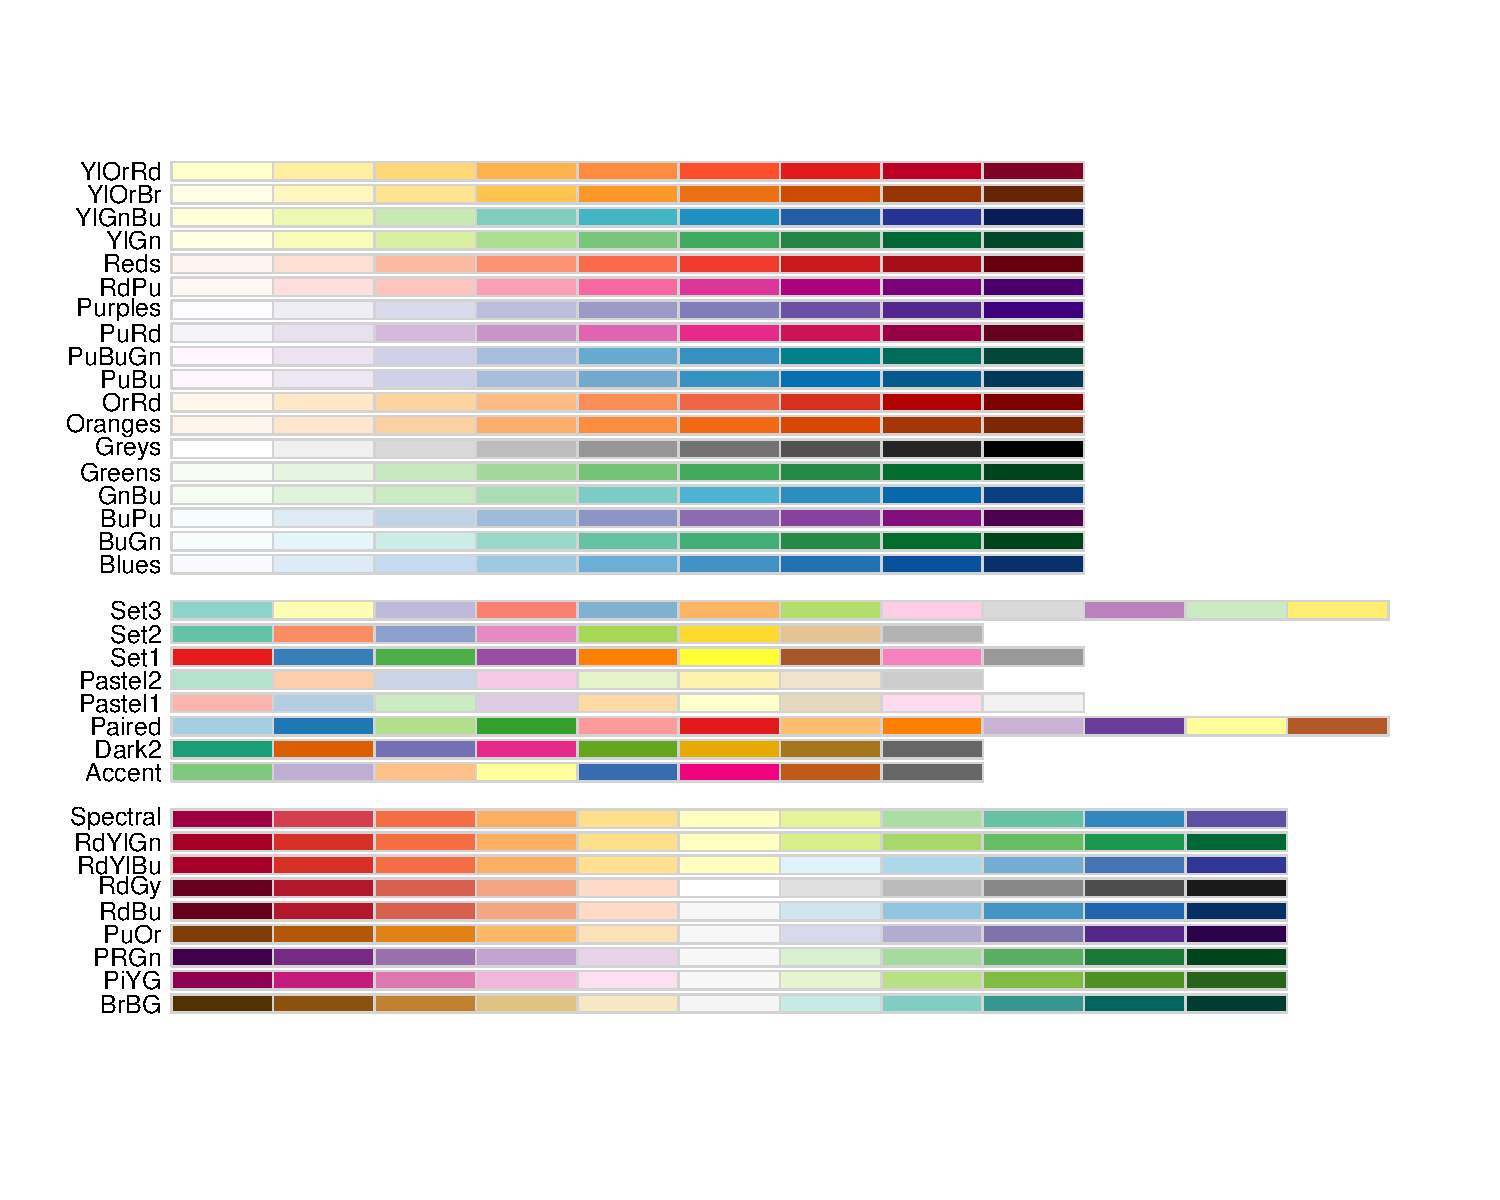
\includegraphics[width=.8\linewidth,height=.8\linewidth]{figure/colorbrewer-1} 

}



\end{knitrout}
\end{frame}

%------------------------------------------------

\begin{frame}[fragile]
\frametitle{Brewer palette}
The main function of \code{"RColorBrewer"} is {\hilit \code{brewer.pal()}} that allows you to select a color palette by specifying the name and size of the palette.
\begin{knitrout}\scriptsize
\definecolor{shadecolor}{rgb}{0.969, 0.969, 0.969}\color{fgcolor}\begin{kframe}
\begin{alltt}
\hlcom{# palette "BuPu" (blue-purple)}
\hlstd{n} \hlkwb{<-} \hlnum{7}
\hlkwd{pie}\hlstd{(}\hlkwd{rep}\hlstd{(}\hlnum{1}\hlstd{, n),} \hlkwc{col} \hlstd{=} \hlkwd{brewer.pal}\hlstd{(n,} \hlstr{"BuPu"}\hlstd{))}
\end{alltt}
\end{kframe}

{\centering 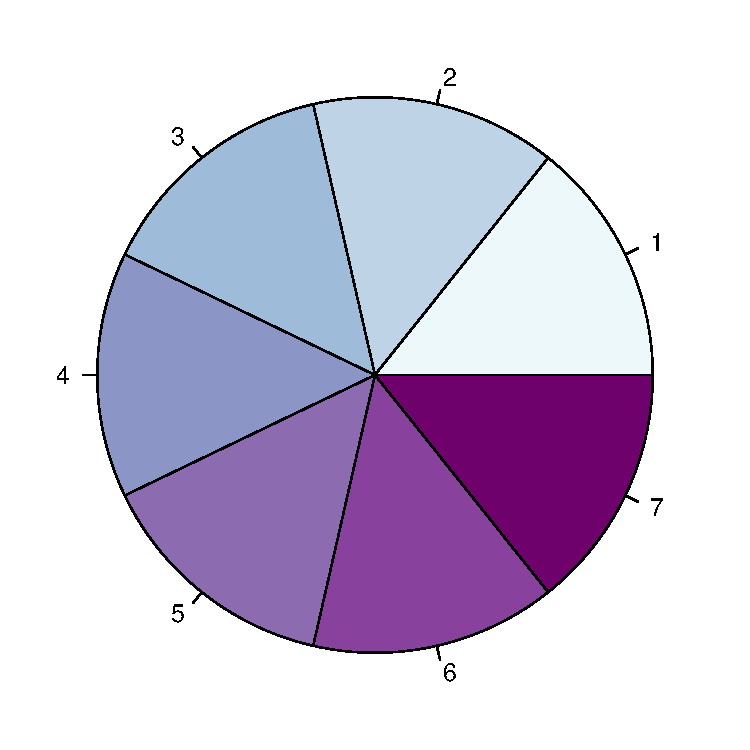
\includegraphics[width=.4\linewidth,height=.4\linewidth]{figure/brewerpal-1} 

}



\end{knitrout}
\end{frame}

%------------------------------------------------

\begin{frame}[fragile]
\frametitle{Brewer palette}
\begin{knitrout}\scriptsize
\definecolor{shadecolor}{rgb}{0.969, 0.969, 0.969}\color{fgcolor}\begin{kframe}
\begin{alltt}
\hlcom{# palette "Spectral"}
\hlstd{n} \hlkwb{<-} \hlnum{11}
\hlkwd{pie}\hlstd{(}\hlkwd{rep}\hlstd{(}\hlnum{1}\hlstd{, n),} \hlkwc{col} \hlstd{=} \hlkwd{brewer.pal}\hlstd{(n,} \hlstr{"Spectral"}\hlstd{))}
\end{alltt}
\end{kframe}

{\centering 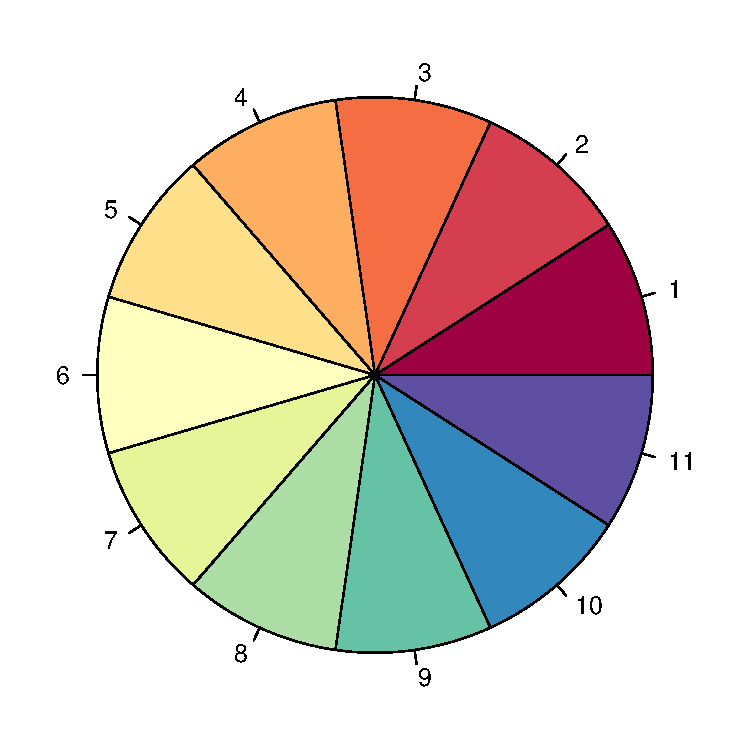
\includegraphics[width=.4\linewidth,height=.4\linewidth]{figure/spectral-1} 

}



\end{knitrout}
\end{frame}

%------------------------------------------------

\begin{frame}[fragile]
\frametitle{More about color spaces}

\bi 
 \item The package \code{"colorspace"} provides functions to create colors in a variety of color spaces, plus functions to convert between color spaces.
 \item Another useful package is \code{"munsell"}, which is designed on the Munsell color space.
 \item There is also the \code{"dichromat"} package that provides a series of palettes that are suitable for people with color blindness deficiencies.
\ei

\end{frame}

%------------------------------------------------

\begin{frame}
\begin{center}
\Huge{\hilit{Color Wheel}}
\end{center}
\end{frame}

%------------------------------------------------

\begin{frame}[fragile]
\frametitle{Color Wheel}

\bb{Understanding the Color Wheel}
The color wheel helps you visualize the relationships that colors have to one another. The wheel shows different colors evenly apart.
\eb

\begin{knitrout}\scriptsize
\definecolor{shadecolor}{rgb}{0.969, 0.969, 0.969}\color{fgcolor}

{\centering 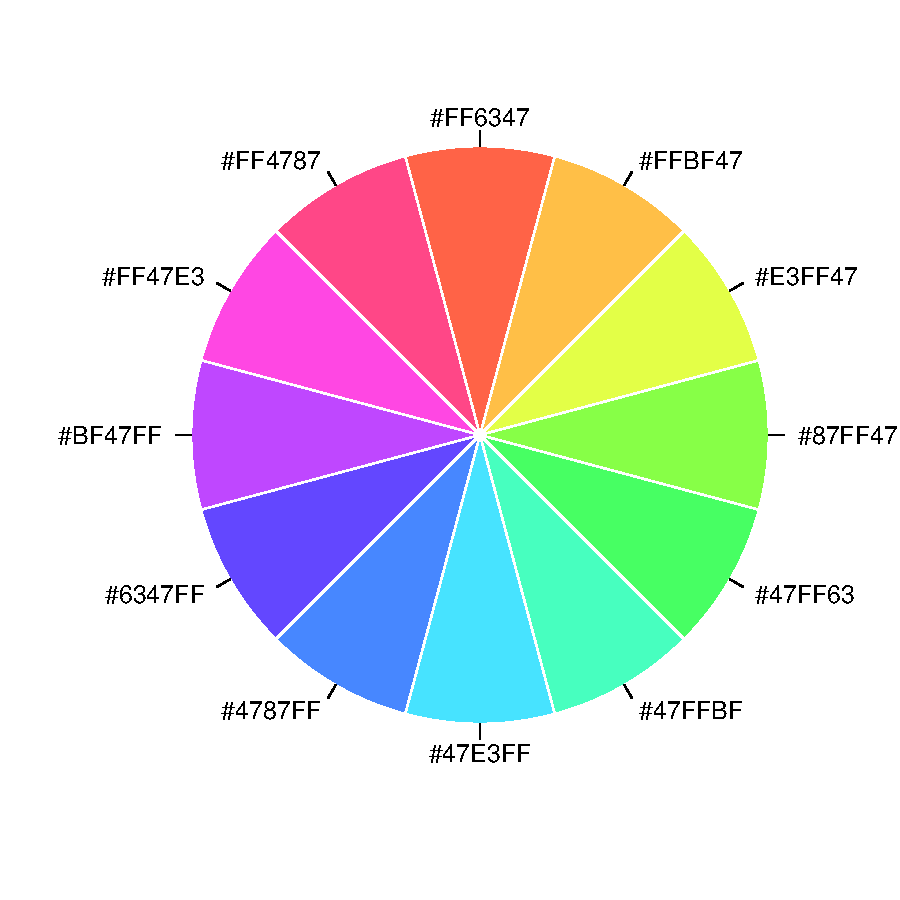
\includegraphics[width=.4\linewidth,height=.4\linewidth]{figure/colorwheel-1} 

}



\end{knitrout}

\end{frame}

%------------------------------------------------

\begin{frame}[fragile]
\frametitle{Color Wheel}

The R package \code{"colortools"} provides the function {\hilit \code{wheel()}}. The function takes the name of a color, and produces a corresponding color wheel with the specified number of slices. 

\begin{knitrout}\tiny
\definecolor{shadecolor}{rgb}{0.969, 0.969, 0.969}\color{fgcolor}\begin{kframe}
\begin{alltt}
\hlcom{# remember to install colortools first!}
\hlkwd{library}\hlstd{(colortools)}
\hlcom{# color wheel for 'tomato'}
\hlkwd{wheel}\hlstd{(}\hlstr{"#FFB973"}\hlstd{,} \hlkwc{bg} \hlstd{=} \hlstr{"white"}\hlstd{)}
\end{alltt}
\end{kframe}

{\centering 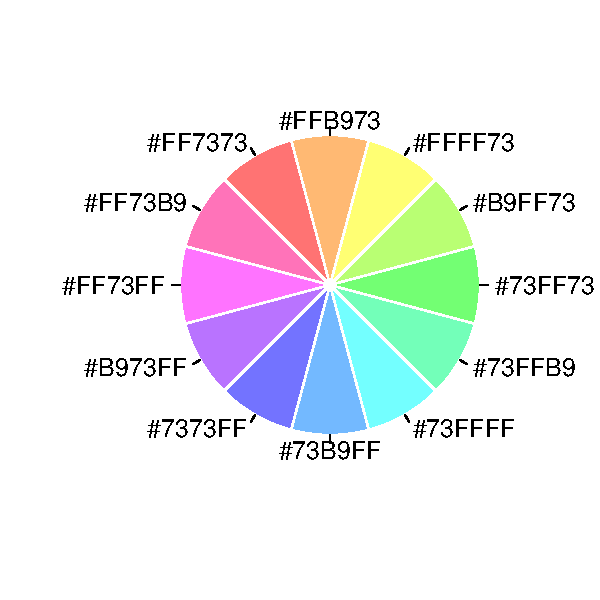
\includegraphics[width=.3\linewidth,height=.3\linewidth]{figure/tomato_wheel-1} 

}


\begin{kframe}\begin{verbatim}
##  [1] "#FFB973" "#FFFF73" "#B9FF73" "#73FF73" "#73FFB9" "#73FFFF" "#73B9FF"
##  [8] "#7373FF" "#B973FF" "#FF73FF" "#FF73B9" "#FF7373"
\end{verbatim}
\end{kframe}
\end{knitrout}

\end{frame}

%------------------------------------------------

\begin{frame}[fragile]

\begin{columns}[t]
\begin{column}{0.5\textwidth}
\begin{knitrout}\tiny
\definecolor{shadecolor}{rgb}{0.969, 0.969, 0.969}\color{fgcolor}\begin{kframe}
\begin{alltt}
\hlcom{# Adjacent (analogous)}
\hlkwd{adjacent}\hlstd{(}\hlstr{"tomato"}\hlstd{,} \hlkwc{title} \hlstd{=} \hlnum{FALSE}\hlstd{)}
\end{alltt}
\end{kframe}

{\centering 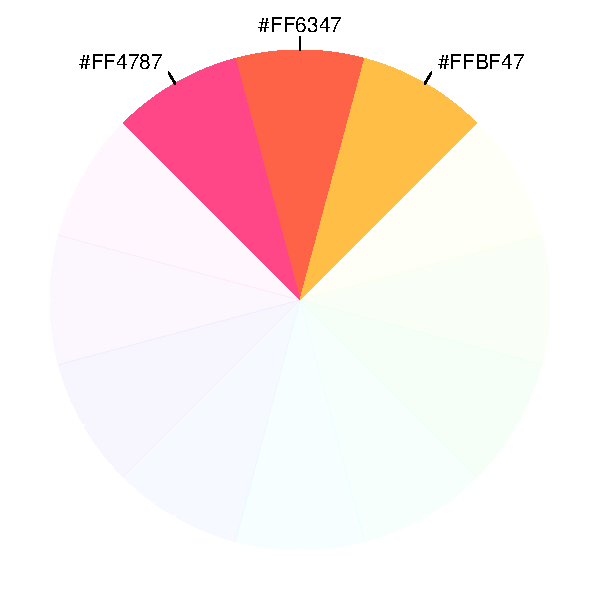
\includegraphics[width=.6\linewidth,height=.6\linewidth]{figure/tomato_adjacent-1} 

}



\end{knitrout}
\end{column}

\begin{column}{0.5\textwidth}
\begin{knitrout}\tiny
\definecolor{shadecolor}{rgb}{0.969, 0.969, 0.969}\color{fgcolor}\begin{kframe}
\begin{alltt}
\hlcom{# Complementary}
\hlkwd{complementary}\hlstd{(}\hlstr{"tomato"}\hlstd{,} \hlkwc{title} \hlstd{=} \hlnum{FALSE}\hlstd{)}
\end{alltt}
\end{kframe}

{\centering 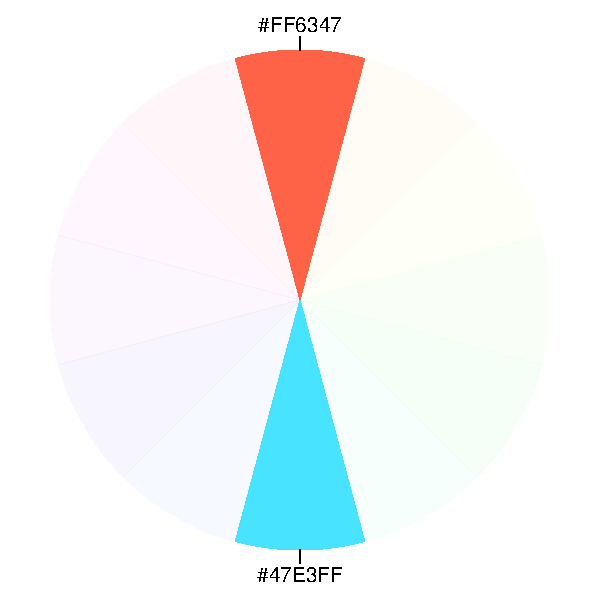
\includegraphics[width=.6\linewidth,height=.6\linewidth]{figure/tomato_complementary-1} 

}



\end{knitrout}
\end{column}
\end{columns}

\end{frame}

%------------------------------------------------

\begin{frame}[fragile]

\begin{columns}[t]
\begin{column}{0.5\textwidth}
\begin{knitrout}\tiny
\definecolor{shadecolor}{rgb}{0.969, 0.969, 0.969}\color{fgcolor}\begin{kframe}
\begin{alltt}
\hlcom{# split complementary}
\hlkwd{splitComp}\hlstd{(}\hlstr{"tomato"}\hlstd{,} \hlkwc{title} \hlstd{=} \hlnum{FALSE}\hlstd{)}
\end{alltt}
\end{kframe}

{\centering 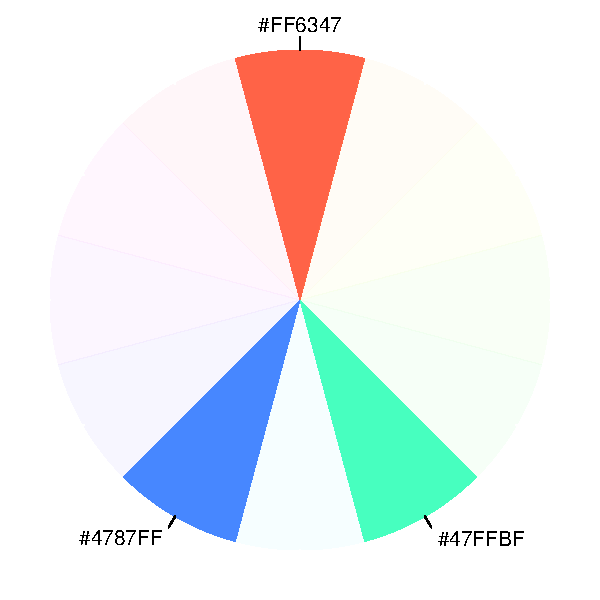
\includegraphics[width=.6\linewidth,height=.6\linewidth]{figure/tomato_split-1} 

}



\end{knitrout}
\end{column}

\begin{column}{0.5\textwidth}
\begin{knitrout}\tiny
\definecolor{shadecolor}{rgb}{0.969, 0.969, 0.969}\color{fgcolor}\begin{kframe}
\begin{alltt}
\hlcom{# triadic}
\hlkwd{triadic}\hlstd{(}\hlstr{"tomato"}\hlstd{,} \hlkwc{title} \hlstd{=} \hlnum{FALSE}\hlstd{)}
\end{alltt}
\end{kframe}

{\centering 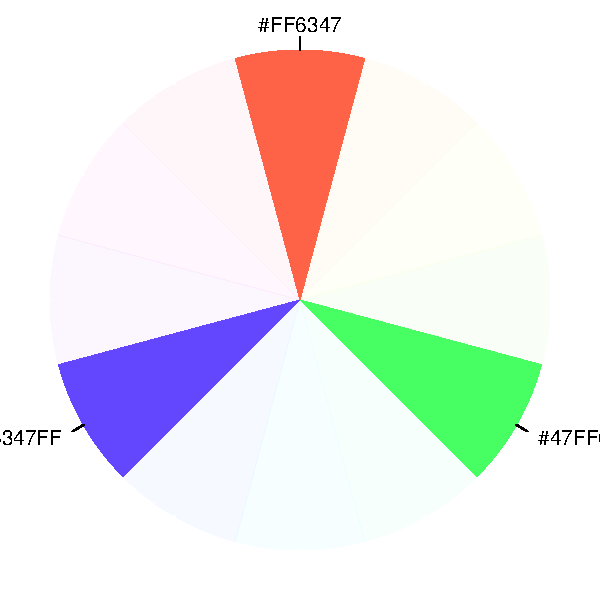
\includegraphics[width=.6\linewidth,height=.6\linewidth]{figure/tomato_triadic-1} 

}



\end{knitrout}
\end{column}
\end{columns}

\end{frame}

%------------------------------------------------

\begin{frame}[fragile]

\begin{columns}[t]
\begin{column}{0.5\textwidth}
\begin{knitrout}\tiny
\definecolor{shadecolor}{rgb}{0.969, 0.969, 0.969}\color{fgcolor}\begin{kframe}
\begin{alltt}
\hlcom{# tetradic}
\hlkwd{tetradic}\hlstd{(}\hlstr{"tomato"}\hlstd{,} \hlkwc{title} \hlstd{=} \hlnum{FALSE}\hlstd{)}
\end{alltt}
\end{kframe}

{\centering 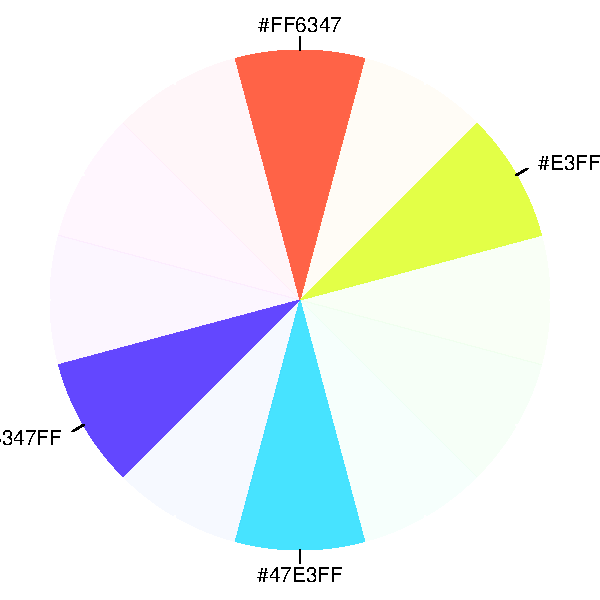
\includegraphics[width=.6\linewidth,height=.6\linewidth]{figure/tomato_tetradic-1} 

}



\end{knitrout}
\end{column}

\begin{column}{0.5\textwidth}
\begin{knitrout}\tiny
\definecolor{shadecolor}{rgb}{0.969, 0.969, 0.969}\color{fgcolor}\begin{kframe}
\begin{alltt}
\hlcom{# square}
\hlkwd{square}\hlstd{(}\hlstr{"tomato"}\hlstd{,} \hlkwc{title} \hlstd{=} \hlnum{FALSE}\hlstd{)}
\end{alltt}
\end{kframe}

{\centering 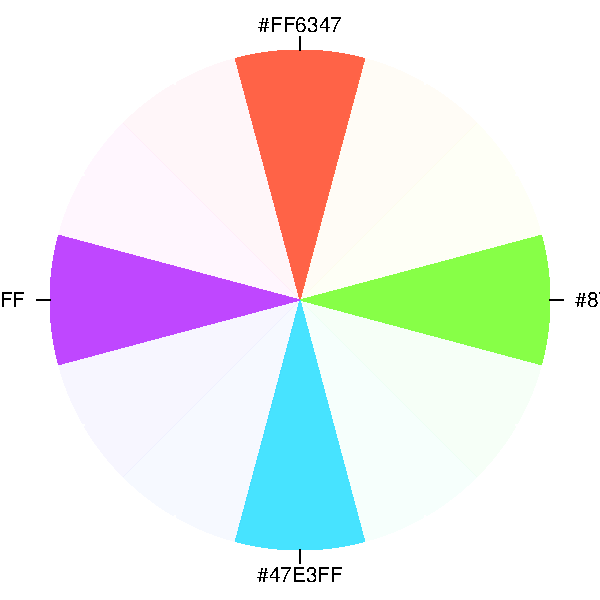
\includegraphics[width=.6\linewidth,height=.6\linewidth]{figure/tomato_square-1} 

}



\end{knitrout}
\end{column}
\end{columns}

\end{frame}

%------------------------------------------------

\begin{frame}
\frametitle{Ramp Palettes}

\bb{\code{colorRampPalette()}}
R also offers the functions \code{colorRamp()} and \code{colorRampPalette()}. They are not color set generators, but color set \textbf{function} generators.
\eb

\end{frame}

%------------------------------------------------

\begin{frame}[fragile]
\frametitle{Ramp Palettes}

\bb{\code{colorRamp()}}
\code{colorRamp()} produces a function for creating colors based on a sequence of values in the range 0 to 1. The output is a numeric matrix of RGB color values
\begin{knitrout}\footnotesize
\definecolor{shadecolor}{rgb}{0.969, 0.969, 0.969}\color{fgcolor}\begin{kframe}
\begin{alltt}
\hlstd{red_green} \hlkwb{<-} \hlkwd{colorRamp}\hlstd{(}\hlkwd{c}\hlstd{(}\hlstr{"red"}\hlstd{,} \hlstr{"green"}\hlstd{))}
\hlkwd{red_green}\hlstd{( (}\hlnum{0}\hlopt{:}\hlnum{4}\hlstd{)}\hlopt{/}\hlnum{4} \hlstd{)}
\end{alltt}
\begin{verbatim}
##        [,1]   [,2] [,3]
## [1,] 255.00   0.00    0
## [2,] 191.25  63.75    0
## [3,] 127.50 127.50    0
## [4,]  63.75 191.25    0
## [5,]   0.00 255.00    0
\end{verbatim}
\end{kframe}
\end{knitrout}
\eb

\end{frame}

%------------------------------------------------

\begin{frame}[fragile]
\frametitle{Ramp Palettes}

\bb{\code{colorRampPalette()}}
\code{colorRampPalette()} produces a function that generates \code{n} colors
\begin{knitrout}\footnotesize
\definecolor{shadecolor}{rgb}{0.969, 0.969, 0.969}\color{fgcolor}\begin{kframe}
\begin{alltt}
\hlstd{orange_blue} \hlkwb{<-} \hlkwd{colorRampPalette}\hlstd{(}\hlkwd{c}\hlstd{(}\hlstr{"orange"}\hlstd{,} \hlstr{"blue"}\hlstd{))}
\hlkwd{orange_blue}\hlstd{(}\hlnum{5}\hlstd{)}
\end{alltt}
\begin{verbatim}
## [1] "#FFA500" "#BF7B3F" "#7F527F" "#3F29BF" "#0000FF"
\end{verbatim}
\end{kframe}
\end{knitrout}
\eb

\end{frame}

%------------------------------------------------

\begin{frame}
\frametitle{Colors and Graphic Devices}

\bb{Color appearance}
The final appearance of a color can vary considerably depending on whether it appears on a screen, printed on paper, or displayed through a projector.
\eb

\bb{Device Dependency of Color}
The colors that R sends to a graphics device are \textbf{sRGB} colors; the reason is that most computer monitors are set up to work with sRGB model.
\eb

\end{frame}

%------------------------------------------------

\begin{frame}
\frametitle{Some Resources}

\bbi
  \item Color-Hex \\
  \url{http://www.color-hex.com/}
  \item Paletton \\
  \url{http://paletton.com}
  \item Adobe color scheme \\
  \url{https://color.adobe.com/create/color-wheel/}
\ei

\end{frame}

%------------------------------------------------

\begin{frame}
\begin{center}
\ig[width=10cm]{images/colorhex.png}
\end{center}
\end{frame}

%------------------------------------------------

\begin{frame}
\begin{center}
\ig[width=11cm]{images/paletton.png}
\end{center}
\end{frame}

%------------------------------------------------

\begin{frame}
\begin{center}
\ig[width=11cm]{images/adobecolor.png}
\end{center}
\end{frame}

%------------------------------------------------

\end{document}
